% Options for packages loaded elsewhere
% Options for packages loaded elsewhere
\PassOptionsToPackage{unicode}{hyperref}
\PassOptionsToPackage{hyphens}{url}
\PassOptionsToPackage{dvipsnames,svgnames,x11names}{xcolor}
%
\documentclass[
  chinese,
]{ctexart}
\usepackage{xcolor}
\usepackage[margin=1in]{geometry}
\usepackage{amsmath,amssymb}
\setcounter{secnumdepth}{-\maxdimen} % remove section numbering
\usepackage{iftex}
\ifPDFTeX
  \usepackage[T1]{fontenc}
  \usepackage[utf8]{inputenc}
  \usepackage{textcomp} % provide euro and other symbols
\else % if luatex or xetex
  \usepackage{unicode-math} % this also loads fontspec
  \defaultfontfeatures{Scale=MatchLowercase}
  \defaultfontfeatures[\rmfamily]{Ligatures=TeX,Scale=1}
\fi
\usepackage{lmodern}
\ifPDFTeX\else
  % xetex/luatex font selection
\fi
% Use upquote if available, for straight quotes in verbatim environments
\IfFileExists{upquote.sty}{\usepackage{upquote}}{}
\IfFileExists{microtype.sty}{% use microtype if available
  \usepackage[]{microtype}
  \UseMicrotypeSet[protrusion]{basicmath} % disable protrusion for tt fonts
}{}
\makeatletter
\@ifundefined{KOMAClassName}{% if non-KOMA class
  \IfFileExists{parskip.sty}{%
    \usepackage{parskip}
  }{% else
    \setlength{\parindent}{0pt}
    \setlength{\parskip}{6pt plus 2pt minus 1pt}}
}{% if KOMA class
  \KOMAoptions{parskip=half}}
\makeatother
% Make \paragraph and \subparagraph free-standing
\makeatletter
\ifx\paragraph\undefined\else
  \let\oldparagraph\paragraph
  \renewcommand{\paragraph}{
    \@ifstar
      \xxxParagraphStar
      \xxxParagraphNoStar
  }
  \newcommand{\xxxParagraphStar}[1]{\oldparagraph*{#1}\mbox{}}
  \newcommand{\xxxParagraphNoStar}[1]{\oldparagraph{#1}\mbox{}}
\fi
\ifx\subparagraph\undefined\else
  \let\oldsubparagraph\subparagraph
  \renewcommand{\subparagraph}{
    \@ifstar
      \xxxSubParagraphStar
      \xxxSubParagraphNoStar
  }
  \newcommand{\xxxSubParagraphStar}[1]{\oldsubparagraph*{#1}\mbox{}}
  \newcommand{\xxxSubParagraphNoStar}[1]{\oldsubparagraph{#1}\mbox{}}
\fi
\makeatother

\usepackage{color}
\usepackage{fancyvrb}
\newcommand{\VerbBar}{|}
\newcommand{\VERB}{\Verb[commandchars=\\\{\}]}
\DefineVerbatimEnvironment{Highlighting}{Verbatim}{commandchars=\\\{\}}
% Add ',fontsize=\small' for more characters per line
\usepackage{framed}
\definecolor{shadecolor}{RGB}{241,243,245}
\newenvironment{Shaded}{\begin{snugshade}}{\end{snugshade}}
\newcommand{\AlertTok}[1]{\textcolor[rgb]{0.68,0.00,0.00}{#1}}
\newcommand{\AnnotationTok}[1]{\textcolor[rgb]{0.37,0.37,0.37}{#1}}
\newcommand{\AttributeTok}[1]{\textcolor[rgb]{0.40,0.45,0.13}{#1}}
\newcommand{\BaseNTok}[1]{\textcolor[rgb]{0.68,0.00,0.00}{#1}}
\newcommand{\BuiltInTok}[1]{\textcolor[rgb]{0.00,0.23,0.31}{#1}}
\newcommand{\CharTok}[1]{\textcolor[rgb]{0.13,0.47,0.30}{#1}}
\newcommand{\CommentTok}[1]{\textcolor[rgb]{0.37,0.37,0.37}{#1}}
\newcommand{\CommentVarTok}[1]{\textcolor[rgb]{0.37,0.37,0.37}{\textit{#1}}}
\newcommand{\ConstantTok}[1]{\textcolor[rgb]{0.56,0.35,0.01}{#1}}
\newcommand{\ControlFlowTok}[1]{\textcolor[rgb]{0.00,0.23,0.31}{\textbf{#1}}}
\newcommand{\DataTypeTok}[1]{\textcolor[rgb]{0.68,0.00,0.00}{#1}}
\newcommand{\DecValTok}[1]{\textcolor[rgb]{0.68,0.00,0.00}{#1}}
\newcommand{\DocumentationTok}[1]{\textcolor[rgb]{0.37,0.37,0.37}{\textit{#1}}}
\newcommand{\ErrorTok}[1]{\textcolor[rgb]{0.68,0.00,0.00}{#1}}
\newcommand{\ExtensionTok}[1]{\textcolor[rgb]{0.00,0.23,0.31}{#1}}
\newcommand{\FloatTok}[1]{\textcolor[rgb]{0.68,0.00,0.00}{#1}}
\newcommand{\FunctionTok}[1]{\textcolor[rgb]{0.28,0.35,0.67}{#1}}
\newcommand{\ImportTok}[1]{\textcolor[rgb]{0.00,0.46,0.62}{#1}}
\newcommand{\InformationTok}[1]{\textcolor[rgb]{0.37,0.37,0.37}{#1}}
\newcommand{\KeywordTok}[1]{\textcolor[rgb]{0.00,0.23,0.31}{\textbf{#1}}}
\newcommand{\NormalTok}[1]{\textcolor[rgb]{0.00,0.23,0.31}{#1}}
\newcommand{\OperatorTok}[1]{\textcolor[rgb]{0.37,0.37,0.37}{#1}}
\newcommand{\OtherTok}[1]{\textcolor[rgb]{0.00,0.23,0.31}{#1}}
\newcommand{\PreprocessorTok}[1]{\textcolor[rgb]{0.68,0.00,0.00}{#1}}
\newcommand{\RegionMarkerTok}[1]{\textcolor[rgb]{0.00,0.23,0.31}{#1}}
\newcommand{\SpecialCharTok}[1]{\textcolor[rgb]{0.37,0.37,0.37}{#1}}
\newcommand{\SpecialStringTok}[1]{\textcolor[rgb]{0.13,0.47,0.30}{#1}}
\newcommand{\StringTok}[1]{\textcolor[rgb]{0.13,0.47,0.30}{#1}}
\newcommand{\VariableTok}[1]{\textcolor[rgb]{0.07,0.07,0.07}{#1}}
\newcommand{\VerbatimStringTok}[1]{\textcolor[rgb]{0.13,0.47,0.30}{#1}}
\newcommand{\WarningTok}[1]{\textcolor[rgb]{0.37,0.37,0.37}{\textit{#1}}}

\usepackage{longtable,booktabs,array}
\newcounter{none} % for unnumbered tables
\usepackage{calc} % for calculating minipage widths
% Correct order of tables after \paragraph or \subparagraph
\usepackage{etoolbox}
\makeatletter
\patchcmd\longtable{\par}{\if@noskipsec\mbox{}\fi\par}{}{}
\makeatother
% Allow footnotes in longtable head/foot
\IfFileExists{footnotehyper.sty}{\usepackage{footnotehyper}}{\usepackage{footnote}}
\makesavenoteenv{longtable}
\usepackage{graphicx}
\makeatletter
\newsavebox\pandoc@box
\newcommand*\pandocbounded[1]{% scales image to fit in text height/width
  \sbox\pandoc@box{#1}%
  \Gscale@div\@tempa{\textheight}{\dimexpr\ht\pandoc@box+\dp\pandoc@box\relax}%
  \Gscale@div\@tempb{\linewidth}{\wd\pandoc@box}%
  \ifdim\@tempb\p@<\@tempa\p@\let\@tempa\@tempb\fi% select the smaller of both
  \ifdim\@tempa\p@<\p@\scalebox{\@tempa}{\usebox\pandoc@box}%
  \else\usebox{\pandoc@box}%
  \fi%
}
% Set default figure placement to htbp
\def\fps@figure{htbp}
\makeatother



\ifLuaTeX
\usepackage[bidi=basic,shorthands=off,provide=*]{babel}
\else
\usepackage[bidi=default,shorthands=off,provide=*]{babel}
\fi
\ifLuaTeX
  \usepackage{selnolig} % disable illegal ligatures
\fi


\setlength{\emergencystretch}{3em} % prevent overfull lines

\providecommand{\tightlist}{%
  \setlength{\itemsep}{0pt}\setlength{\parskip}{0pt}}



 


\usepackage{fvextra}
\DefineVerbatimEnvironment{Highlighting}{Verbatim}{breaklines,breakanywhere,commandchars=\\\{\}}
\usepackage{array}
\usepackage{booktabs}
\usepackage{longtable}
\usepackage{tabularx}
\newcolumntype{Y}{>{\raggedright\arraybackslash}X}
\usepackage{changepage}
\usepackage{xcolor}
\makeatletter
\@ifpackageloaded{caption}{}{\usepackage{caption}}
\AtBeginDocument{%
\ifdefined\contentsname
  \renewcommand*\contentsname{目录}
\else
  \newcommand\contentsname{目录}
\fi
\ifdefined\listfigurename
  \renewcommand*\listfigurename{图索引}
\else
  \newcommand\listfigurename{图索引}
\fi
\ifdefined\listtablename
  \renewcommand*\listtablename{表索引}
\else
  \newcommand\listtablename{表索引}
\fi
\ifdefined\figurename
  \renewcommand*\figurename{图}
\else
  \newcommand\figurename{图}
\fi
\ifdefined\tablename
  \renewcommand*\tablename{表}
\else
  \newcommand\tablename{表}
\fi
}
\@ifpackageloaded{float}{}{\usepackage{float}}
\floatstyle{ruled}
\@ifundefined{c@chapter}{\newfloat{codelisting}{h}{lop}}{\newfloat{codelisting}{h}{lop}[chapter]}
\floatname{codelisting}{列表}
\newcommand*\listoflistings{\listof{codelisting}{列表索引}}
\makeatother
\makeatletter
\makeatother
\makeatletter
\@ifpackageloaded{caption}{}{\usepackage{caption}}
\@ifpackageloaded{subcaption}{}{\usepackage{subcaption}}
\makeatother
\usepackage{bookmark}
\IfFileExists{xurl.sty}{\usepackage{xurl}}{} % add URL line breaks if available
\urlstyle{same}
% fallback for those not using the hyperref driver hyperxmp:
\makeatletter
\@ifundefined{xmpquote}{\newcommand{\xmpquote}[1]{#1}}{}
\makeatother
\hypersetup{
  pdftitle={第14讲 强化学习入门：从策略梯度到 PPO，让宇树 G1 自己学会动},
  pdflang={zh-CN},
  colorlinks=true,
  linkcolor={blue},
  filecolor={Maroon},
  citecolor={Blue},
  urlcolor={Blue},
  pdfcreator={LaTeX via pandoc}}


\title{第14讲 强化学习入门：从策略梯度到 PPO，让宇树 G1 自己学会动}
\author{}
\date{}
\begin{document}
\maketitle

\renewcommand*\contentsname{目录}
{
\setcounter{tocdepth}{3}
\tableofcontents
}

从第8讲开始，我们做的事情其实只有一件：训练一个\textbf{策略}，再把它部署到闭环里。第8讲立起了这个概念------策略就是从观测到动作的映射；第9到12讲围着它转了一整圈：采数据、用
ACT 和 VLA
学它、微调它；第13讲看了它的前沿形态。这一整段有个共同前提：\textbf{训练信号来自人的示教}------每一步都有人告诉网络''该做什么''。

这一讲把这个前提抽掉。有些事情示教教不了：没人能遥操作出人形机器人 29
个关节的行走节奏；示教信号只说''这一步该做什么''，不说''哪种做法回报更高''；走到示教没覆盖的状态更是无人可问。于是换一种监督信号：不再给''标准答案''，只给一个\textbf{能打分的奖励}，让机器人自己\textbf{试错}。这就是强化学习（Reinforcement
Learning, RL）。

强化学习的概念和算法出了名的多而杂，这一讲不求全，只把入门必须的一条主线走透：先把''学走路''这个任务翻译成强化学习的语言，再建立一张\textbf{不会混淆的方法分类地图}，然后沿着地图上''基于策略''这一支，从最朴素的
REINFORCE
出发，每讲完一个算法就在\textbf{同一个任务}上跑给你看------看到它的毛病，再引出下一个算法------一路升级到工业级的
PPO。最后把同一套 PPO
原样搬去做更难的动作跟随，看看这套配方离开入门任务还剩多少本事。

\section{1 从模仿到试错}\label{ux4eceux6a21ux4effux5230ux8bd5ux9519}

\subsection{1.1
回顾第8讲：策略是从观测到动作的映射}\label{ux56deux987eux7b2c8ux8bb2ux7b56ux7565ux662fux4eceux89c2ux6d4bux5230ux52a8ux4f5cux7684ux6620ux5c04}

第8讲 2.1 节给策略下过定义：\(\pi_\theta\) 是一个参数为 \(\theta\)
的网络，输入观测 \(o_t\)，输出动作
\(a_t\)；部署时它在闭环里反复''看一眼、动一下''。之后几讲无论模型怎么变------ACT、\(\pi_0\)、VLA------都没有离开这个框架，变的只是网络结构和训练数据。

本讲的主角\textbf{还是同一个
\(\pi_\theta\)}，甚至连''闭环交互''这个舞台都没换。真正换掉的只有一样东西：训练信号。模仿学习的每条训练样本都带着''这一步该做什么''的动作标签；强化学习没有标签，只有环境对结果的打分。

\begin{quote}
备注：符号上有一处小衔接。强化学习教材习惯把策略的输入写成状态
\(s_t\)，第8讲写的是观测
\(o_t\)。区别在于''看没看全''：状态是环境的完整信息（\textbf{完全可观测}），观测是策略实际看到的部分（真机常常只做到\textbf{部分可观测}）。本讲在仿真里把该看的都给了策略，两者暂不区分、统一写
\(s_t\)；真机上''看不全''的麻烦见 2.2 节的备注。
\end{quote}

\subsection{1.2
示教教不了的事}\label{ux793aux6559ux6559ux4e0dux4e86ux7684ux4e8b}

模仿学习的天花板，第8讲和第10讲都碰到过。集中起来是三件事：

\begin{itemize}
\tightlist
\item
  \textbf{有些任务根本采不到合用的示教}。桌面操作可以用主从臂示教（第9讲），但人形行走要
  29
  个关节以每秒几十次的频率协调发力，很难直接采到\textbf{足够覆盖、足够稳定、又能当低层控制标签}的示教数据------主从遥操作这类装置尤其够不着（动捕、动作重定向能提供某种参考动作，但那是另一种监督，6.6
  节就会这么用）。本讲的任务------让 G1 学走路------恰好就是这种情形。
\item
  \textbf{缺少直接优化任务回报的机制}。纯行为克隆的学习目标是''贴近示教动作''，受示教分布与标签质量约束；监督信号里没有''哪种做法回报更高''这个概念。（要注意这不等于''模型上限就是示范者水平''：聚合多个示范者、去噪、泛化，都可能让策略在某些指标上超过单个示范者。真正的限制是数据支持范围、优化目标和评测分布。）
\item
  \textbf{错了不会救}。第8讲 3.2
  节讲过闭环里误差会滚雪球：一旦走到示教数据没覆盖的状态，模型两眼一抹黑，因为那里没有标签。
\end{itemize}

三件事的根源是同一个：模仿学习的监督信号回答的是''\textbf{这一步该做什么}''。而上面三个场景需要的是另一种信号------``\textbf{这一步做得好不好}''。

\subsection{1.3
用奖励代替标签}\label{ux7528ux5956ux52b1ux4ee3ux66ffux6807ux7b7e}

``做得好不好''用一个标量就能表达：\textbf{奖励}。环境每收到一个动作，除了转移到新状态，还吐回一个分数。于是第8讲的部署闭环''观测
→ 动作 → 环境 →
新观测''上多出一条回路：\textbf{每一步都带回一个奖励}。机器人在闭环里反复尝试，把''怎么动能拿高分''自己摸出来。

这个改动顺带改变了 rollout 的身份。第8讲里 rollout
是\textbf{验证工具}------loss 再低也要拉到闭环里跑过才算数；本讲里
rollout
变成了\textbf{训练数据本身}：机器人自己跑出来的轨迹、连同每一步的得分，就是训练集。数据不再是事先采好的静态数据集，而是边训练边生成、随着策略变化而变化------这是强化学习与模仿学习在工程形态上最大的不同，也是后面
3.4 节讨论''这些自产数据怎么用''的伏笔。

\subsection{1.4 本讲的任务与路线：让 G1
学会走路}\label{ux672cux8bb2ux7684ux4efbux52a1ux4e0eux8defux7ebfux8ba9-g1-ux5b66ux4f1aux8d70ux8def}

贯穿全讲的任务只有一个：\textbf{宇树 G1
人形机器人，在平地上按速度指令行走}------每个回合随机给一个目标速度（前进/侧移/转向），走稳、跟上就得分。选它做入门载体有三个理由：它不需要任何示教数据（正是
1.2
节的第一种情形）；``跟上速度、别摔倒''的分数很好写；仿真里可以大规模并行试错，单卡就能复现。

方法上我们走一条\textbf{三级阶梯}，每一级都是一个完整算法，在同一个任务上跑出来对照：

\begin{itemize}
\tightlist
\item
  \textbf{v1
  REINFORCE}：最朴素的策略梯度，能学，但涨得慢、很早见顶、还会摔；
\item
  \textbf{v2
  A2C}：请一个''评分员''（critic）当参照物，把学习信号洗干净，动作幅度明显打开，但时不时被一次更新推坏；
\item
  \textbf{v3 PPO}：给每次更新加上护栏，又稳又省数据------工业级配方。
\end{itemize}

为了让对照干净，三个版本刻意做到\textbf{只有算法不同}：同一个环境、同一个网络结构（\texttt{code/rl/1\_rl\_basics/1\_1\_g1\_walk\_rl/model.py}
里的 \texttt{ActorCritic}）、同一份训练预算（4096 个并行环境 × 每轮 24
步 × 3000 迭代）；评测口径也完全一致------各自的最终权重、确定性动作、16
个环境 × 400 步统一打分。三份训练脚本都用标准的 PyTorch Lightning
结构组织：一个在线采样的 \texttt{Dataset}、一个
\texttt{LightningDataModule}、一个负责算 loss 的
\texttt{LightningModule}，入口统一是
\texttt{trainer.fit(model,\ data)}；要调的超参就写在第一次用到它的地方，改文件里的变量即可。\textbf{版本之间的差异（diff）就是这一讲的知识点}------读懂三个文件的区别，就读懂了从
REINFORCE 到 PPO 的演进。

讲完 PPO，6.6 节还会把同一套代码原样搬到一个难得多的任务------让 G1
逐帧贴住一段真实武术动作------看看同一套算法在硬任务上能做到什么程度。

\section{2
把「学走路」写成强化学习问题}\label{ux628aux5b66ux8d70ux8defux5199ux6210ux5f3aux5316ux5b66ux4e60ux95eeux9898}

强化学习有一套自己的词汇。这一节不空讲定义，每引入一个词，就立刻落到 G1
行走任务上------把''学走路''完整翻译成强化学习的语言，后面所有算法都在这套语言上工作。

\subsection{2.1
智能体与环境：一个回合怎么跑}\label{ux667aux80fdux4f53ux4e0eux73afux5883ux4e00ux4e2aux56deux5408ux600eux4e48ux8dd1}

强化学习的基本场景只有两个角色：一个\textbf{智能体（agent）}在一个\textbf{环境（environment）}里行动。智能体每一步看到环境的状态，做一个动作；环境收到动作后，给出一个奖励、并转移到下一个状态。

\begin{figure}[H]

{\centering 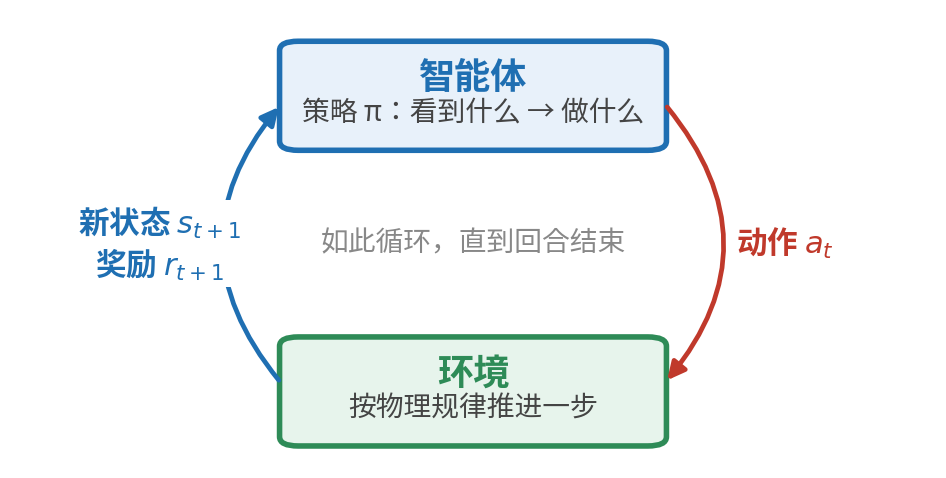
\includegraphics[width=1\linewidth,height=\textheight,keepaspectratio]{../../assets/figures/lecture14/ref/fig141-agent-env-loop.png}

}

\caption{智能体与环境的交互闭环：智能体在状态 \(s_t\) 下输出动作
\(a_t\)，环境返回新的状态 \(s_{t+1}\) 和奖励 \(r_{t+1}\)（``做完 \(a_t\)
之后拿到的那一份''），如此循环}

\end{figure}%

把一步交互写成符号，就是：

\[
s_t \;\xrightarrow{\;a_t\;}\; r_{t+1},\, s_{t+1}
\]

这个抽象框架放到 G1 行走上，每个角色的具体所指是：

\begin{center}
\begin{tabular}{@{}>{\raggedright\arraybackslash}p{\dimexpr 0.3250\linewidth - 2\tabcolsep\relax} >{\raggedright\arraybackslash}p{\dimexpr 0.4104\linewidth - 2\tabcolsep\relax} >{\raggedright\arraybackslash}p{\dimexpr 0.2646\linewidth - 2\tabcolsep\relax}@{}}
\toprule\noalign{}
概念 & 含义 & 在 G1 行走里的具体所指 \\
\midrule\noalign{}
智能体 agent & 做决策的主体 & 控制 G1 的策略网络 \\
环境 environment & 智能体交互的世界 & 仿真器里的物理引擎 \\
状态 state & 环境在这一刻的完整描述（本讲仿真里策略看到的就是它） & 关节角度、躯干姿态、目标速度指令 \\
动作 action & 智能体做出的动作 & 29 个关节的目标量 \\
奖励 reward & 环境返回的反馈 & 跟上速度 + 保持直立 − 各种惩罚 \\
轨迹 trajectory / 回合 episode & 一整段交互 & 从站立开始，到摔倒或 20 秒超时 \\
\bottomrule\noalign{}
\end{tabular}
\end{center}

``试错''的量从哪来？仿真里同时开 \textbf{4096 个并行环境}，4096 台虚拟
G1
同时摔、同时爬起来，一轮就贡献近十万步经验。这是强化学习在仿真里能成的关键工程条件。

\subsection{2.2 状态与动作：G1
看到什么、能动什么}\label{ux72b6ux6001ux4e0eux52a8ux4f5cg1-ux770bux5230ux4ec0ux4e48ux80fdux52a8ux4ec0ux4e48}

智能体''看到什么''叫\textbf{观测空间}，``能做什么''叫\textbf{动作空间}。对入门来说，动作空间的区别尤其要分清：

\begin{figure}[H]

{\centering 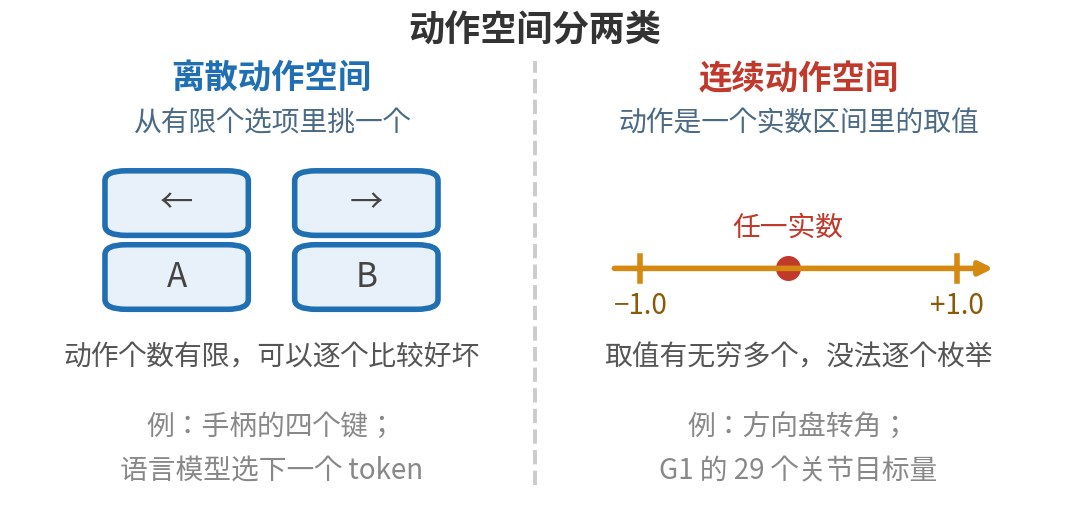
\includegraphics[width=1\linewidth,height=\textheight,keepaspectratio]{../../assets/figures/lecture14/ref/fig-action-space.png}

}

\caption{动作空间分两类。左边是离散：动作是几个方框里挑一个（图上画的是手柄的四个键），数得清，所以可以逐个比较好坏。右边是连续：动作是一根实数轴上的任意一点（图上画的是
−1 到 +1 这段），取值有无穷多个，没法逐个枚举}

\end{figure}%

\begin{itemize}
\tightlist
\item
  \textbf{离散动作空间}：动作是有限个选项里挑一个，比如游戏手柄的几个按键、语言模型从词表里选下一个
  token。
\item
  \textbf{连续动作空间}：动作是一个或一组实数，比如方向盘转角、机械臂每个关节的目标量。
\end{itemize}

G1 的状态是关节角度、躯干姿态加上目标速度指令；动作是 \textbf{29
个关节的目标量，每个都是连续实数}------高维连续动作空间。记住这个事实，3.2
节讲算法分类时它会直接决定我们选哪一支。

\begin{quote}
备注：宇树 G1 有多种关节配置------官方规格表里基础版是 23
个自由度，加上腰部、腕部与三指灵巧手最多到 43 个。本讲全程按 \textbf{29
个关节}算：mjlab 自带的 G1 模型是双腿各 6 个、双臂各 7 个、腰部 3
个，合起来正好 29；重定向管线那边用的 G1 模型文件也是 29
自由度那一版（\texttt{g1\_mocap\_29dof.xml}）。换配置只改这个数字，算法一行不用动。
\end{quote}

\begin{quote}
备注：真实机器人还有一层麻烦------它通常不是''完全可观测''的：相机只看到局部画面，物体可能被遮挡，执行还带误差。这类''看不全''的问题在学术上叫部分可观测（POMDP）。本讲在仿真里把状态给得比较全（1.1
节说的 \(o_t\) 与 \(s_t\) 暂不区分），但要知道真机会更难。
\end{quote}

\subsection{2.3
奖励与回报：怎么给「走得好」打分}\label{ux5956ux52b1ux4e0eux56deux62a5ux600eux4e48ux7ed9ux8d70ux5f97ux597dux6253ux5206}

\textbf{奖励（reward）}是某一步的即时反馈，一个标量。G1
这一帧跟上了目标速度、躯干直立，给正分；动作过猛、关节顶到限位、脚底打滑，扣分。\textbf{怎么设计奖励，是强化学习里最关键也最难的一环}------分数写歪了，机器人就会学出''钻空子''的动作；机器人和大模型任务里奖励还常常很稀疏，很久才有一次明确反馈。行走任务的好处是\textbf{反馈稠密、每步都有}（速度跟踪、姿态稳定、能耗和关节限位惩罚都能就地算出来），比稀疏奖励好写得多；但也别把它想得太轻松------这几项之间的权重怎么配，仍会显著左右最终步态，写''能跑''和写''跑得好看''是两回事。

但训练时我们关心的几乎从来不是单步奖励，而是\textbf{从现在开始、未来一整段能拿到多少总分}，这叫\textbf{回报（return）}。一个只顾眼前奖励的策略会很短视：为了这一帧站直而猛地刹住，下一帧反而摔了。回报逼着策略为长远负责。把未来的奖励加起来、按时间打折扣：

\[
R_t \;=\; r_{t+1} + \gamma\, r_{t+2} + \gamma^2 r_{t+3} + \cdots \;=\; \sum_{k=0}^{\infty}\gamma^{k}\, r_{t+k+1}
\]

公式里的折扣因子 \(\gamma\in[0,1]\) 控制''看多远''：越接近 1
越重视长期，越接近 0
越只顾眼前。但求和式本身看不出它到底把视野截在哪儿------那要看权重
\(\gamma^k\) 衰减得多快。

\begin{figure}[H]

{\centering 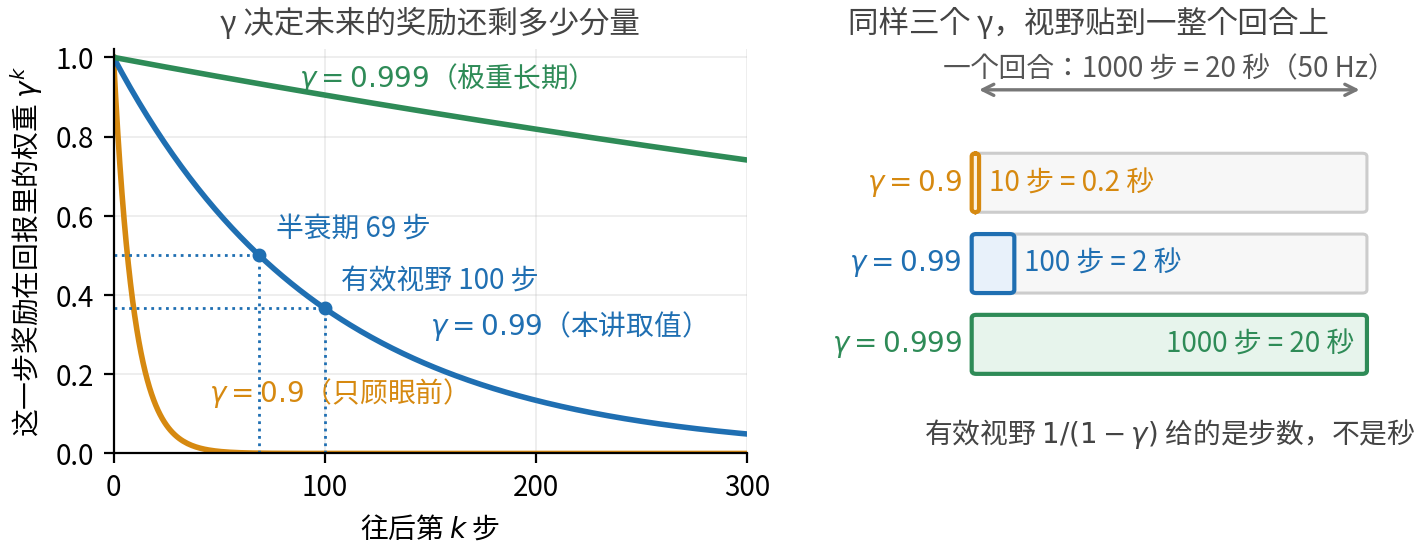
\includegraphics[width=1\linewidth,height=\textheight,keepaspectratio]{../../assets/figures/lecture14/ref/fig14-3-discount-horizon.png}

}

\caption{\(\gamma\) 决定未来的奖励还剩多少分量。左：三个 \(\gamma\)
取值下，往后第 \(k\) 步的奖励在回报里还剩多少权重。本讲取
\(\gamma=0.99\)，半衰期约 69 步（\(0.99^{69}\approx 0.5\)），有效视野
\(1/(1-\gamma)=100\) 步（此处权重已降到
\(0.99^{100}\approx 0.37\)）。右：同样三个 \(\gamma\)
的有效视野贴到一整个回合上------mjlab 的 G1 速度跟随环境仿真步长 0.005
秒、每 4 步出一次动作，即 50 Hz，回合上限 20 秒{[}7{]}，一个回合正好
1000 步}

\end{figure}%

右图那三根条子说明一件容易被忽略的事：\(\gamma=0.99\)
的视野只覆盖一个回合的前十分之一，\textbf{不是''几乎一视同仁地看完整段''}。图下那行小字提醒的坑更要紧------\(1/(1-\gamma)\)
算出来的是\textbf{步数}，不是秒。同一个 0.99，在 50 Hz 的 G1 上折合 2
秒，搬到 200 Hz 的控制回路上就只剩 0.5 秒；换了控制频率却不动
\(\gamma\)，等于悄悄把策略的视野砍掉四分之三。

一句话：\textbf{奖励是每一步的分，回报是一整段的分；强化学习最大化的是回报。}

\subsection{2.4
策略与价值：两个基本量}\label{ux7b56ux7565ux4e0eux4ef7ux503cux4e24ux4e2aux57faux672cux91cf}

\textbf{策略（policy）}沿用第8讲的定义，写成概率形式是
\(\pi_\theta(a\mid s)\)------参数为 \(\theta\) 的网络，在状态 \(s\)
下给出动作 \(a\) 的概率。

\begin{figure}[H]

{\centering 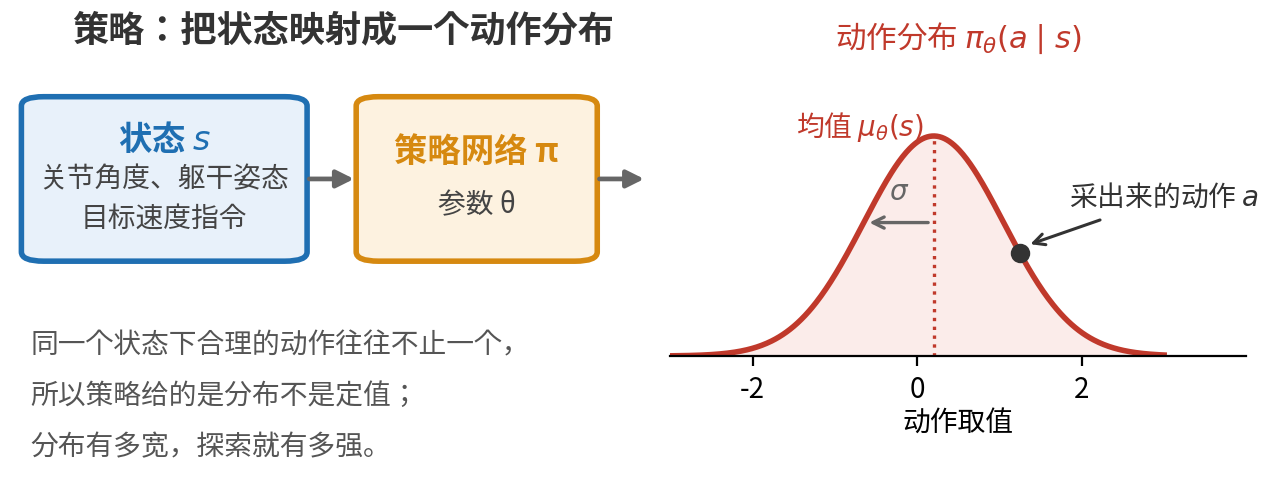
\includegraphics[width=1\linewidth,height=\textheight,keepaspectratio]{../../assets/figures/lecture14/ref/fig14-2-policy-distribution.png}

}

\caption{策略把状态映射成的是一个\textbf{动作分布}，不是一个定值：左边是输入（关节角度、躯干姿态、目标速度指令），中间是参数为
\(\theta\) 的网络，右边是它吐出来的高斯密度------峰值处的均值
\(\mu_\theta(s)\) 是''最想做的动作''，从均值往外量出去的那一段
\(\sigma\) 就是探索强度，黑点是这一步真正采出来去执行的那个
\(a\)。\(\sigma\) 越宽，采到离均值远的动作的机会越大}

\end{figure}%

和第8讲不同的一点是：本讲用\textbf{随机策略}。G1
的策略网络对每个关节吐出高斯分布的\textbf{均值}；标准差不由网络算，而是一组跟着一起训练、但不随状态变化的参数（4.5
节的优化器那一行会再见到它）。训练时从这个分布里\textbf{采样}去试探，部署时直接取均值。随机性是''探索''的来源------不试新动作，就永远不知道有没有更好的走法；这也是试错学习必须付的入场费。

除了策略，强化学习还有第二个基本量：\textbf{价值（value）}------给''一个状态本身有多好''打分的评分员。现在只需要记住有这么个概念：策略负责''怎么做''，价值负责''值多少分''。它的精确定义（\(V\)、\(Q\)、优势
\(A\)）等到第 5 节第一个真正需要它的算法出现时再展开。

\subsection{2.5 本节小结}\label{ux672cux8282ux5c0fux7ed3}

``学走路''翻译成强化学习语言：G1
的策略网络是智能体，物理仿真是环境，每回合随机给速度指令，跟上加分、摔倒扣分；4096
个并行环境提供试错的量。G1 的动作空间是 29 维\textbf{连续}空间。策略
\(\pi_\theta(a\mid s)\) 输出高斯分布、采样探索，目标是最大化折扣回报
\(R_t\) 而非单步奖励；价值是''状态值多少分''的评分员，第 5 节正式登场。

\section{3
强化学习方法分类}\label{ux5f3aux5316ux5b66ux4e60ux65b9ux6cd5ux5206ux7c7b}

概念备齐，先别急着钻算法。强化学习的算法出了名的多------REINFORCE、A2C、TRPO、PPO、DQN、DDPG、SAC、AlphaZero\ldots\ldots 第一次接触很容易被缩写淹没，而且不同教材的分类词还长得很像，一混就乱。这一节把地图画清楚：\textbf{三个互相独立的划分}，每个算法对三个问题各回答一次，就有了自己唯一的坐标。这张地图不但罩住本讲，也罩住后面两讲。

\begin{figure}[H]

{\centering 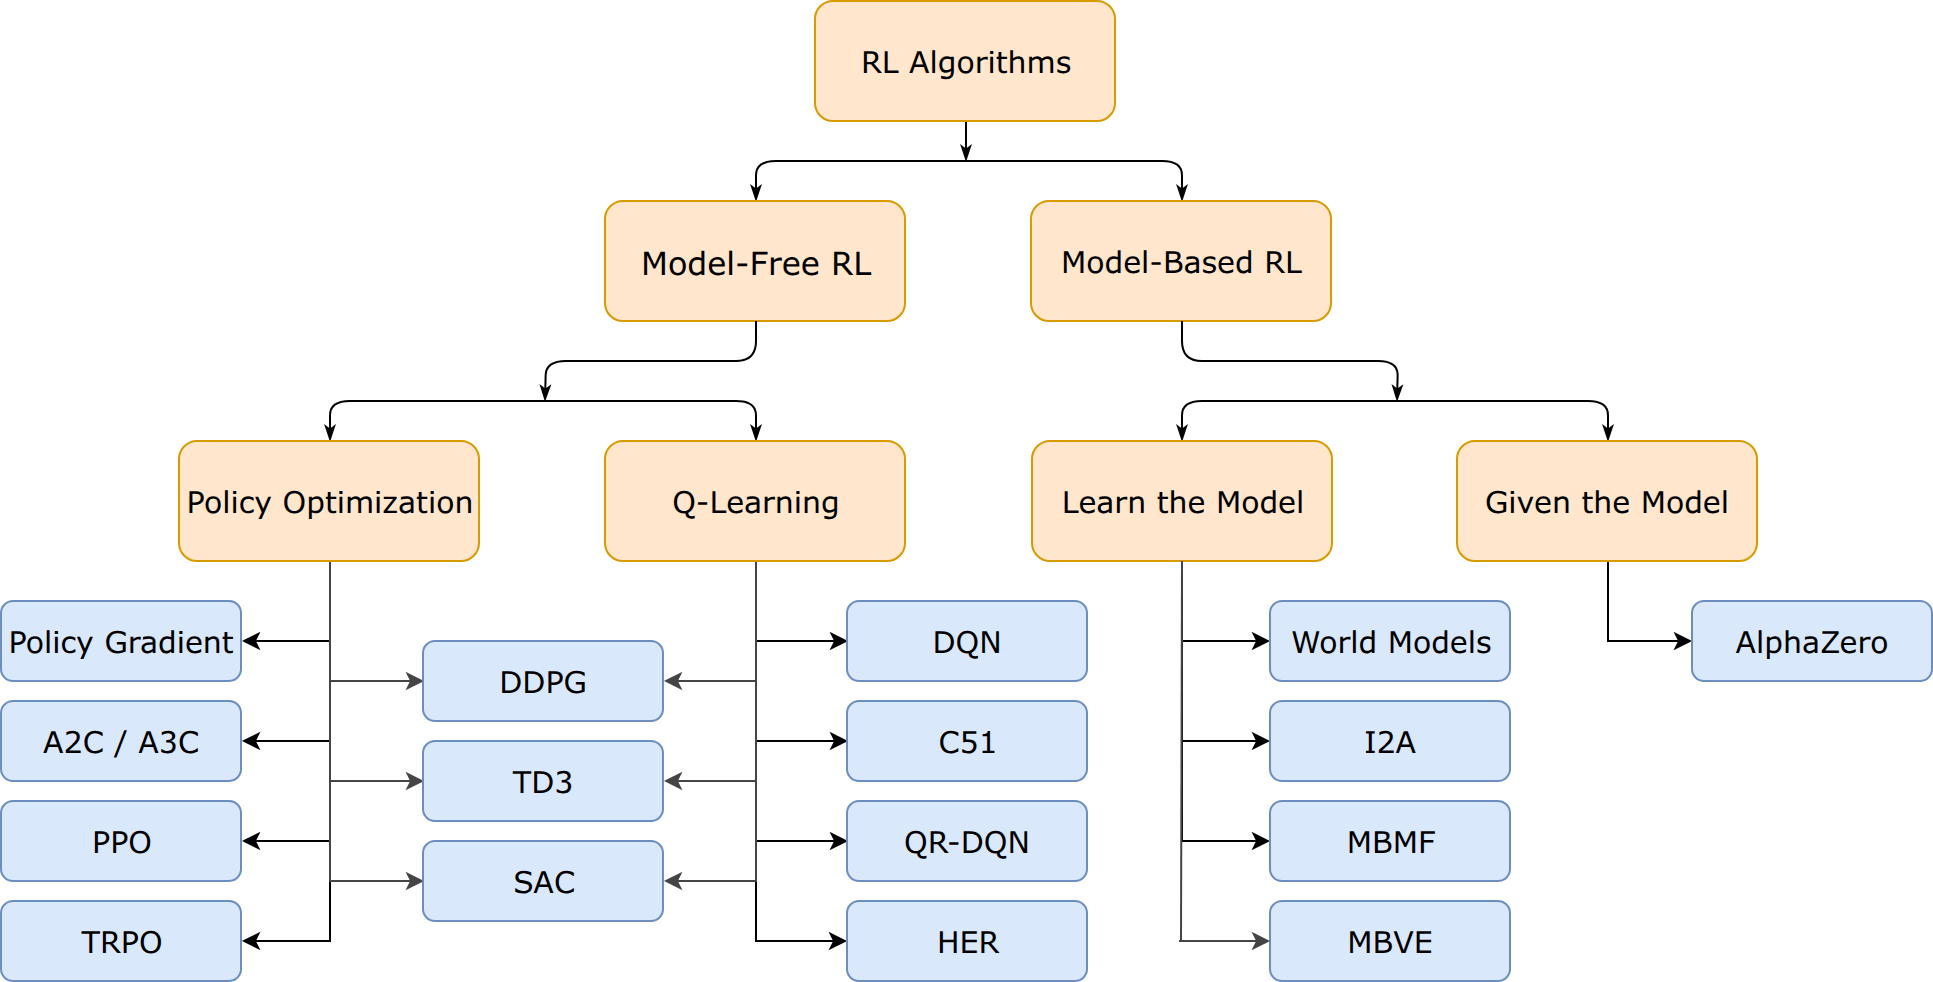
\includegraphics[width=0.94\linewidth,height=\textheight,keepaspectratio]{../../assets/figures/lecture14/ref/fig142-rl-taxonomy.png}

}

\caption{按 Spinning Up
的经典算法分类树{[}1{]}重画（节点与分支逐个对齐原图）：第一层按''学不学环境模型''分成
Model-Free 与 Model-Based；Model-Free 内部按''学什么''分成 Policy
Optimization（基于策略）与 Q-Learning（基于价值）两族，DDPG/TD3/SAC
画在两族之间}

\end{figure}%

\subsection{3.1
第一个划分：学不学环境模型}\label{ux7b2cux4e00ux4e2aux5212ux5206ux5b66ux4e0dux5b66ux73afux5883ux6a21ux578b}

上图的第一刀：\textbf{model-based}
方法先学（或已知）一个''环境会怎么变''的模型，再拿它做规划------图右侧的
World Models、AlphaZero 都在这支。\textbf{model-free}
方法不显式学环境的转移模型、也不用它做规划，直接拿试错经验去更新策略或价值。机器人任务的环境模型（接触、摩擦、碰撞）极难学准，主流走
\textbf{model-free}，即图的左半边------本讲到第16讲的所有算法都在这半边，后面不再讨论
model-based。

\subsection{3.2
第二个划分：学什么------基于价值的方法与基于策略的方法}\label{ux7b2cux4e8cux4e2aux5212ux5206ux5b66ux4ec0ux4e48ux57faux4e8eux4ef7ux503cux7684ux65b9ux6cd5ux4e0eux57faux4e8eux7b56ux7565ux7684ux65b9ux6cd5}

model-free
内部，按''网络到底在学什么''分成两大类。这是整张地图最重要的一刀：

\begin{itemize}
\tightlist
\item
  \textbf{基于价值的方法（value-based）}：不直接学策略，而是学\textbf{动作价值
  \(Q(s,a)\)}------``在状态 \(s\) 做动作
  \(a\)，往后平均能拿多少分''。学好之后，策略是\textbf{导出}的：每一步挑
  \(Q\)
  值最大的动作。这一族的更新工具是贝尔曼方程与\textbf{时序差分}（temporal
  difference,
  TD------用''下一步的估值''回头修''这一步的估值''，第16讲展开），代表算法是
  Q-learning 和它的深度版 DQN------就是分类树 ``Q-Learning'' 那一列。
\item
  \textbf{基于策略的方法（policy-based）}：直接参数化策略
  \(\pi_\theta\)、直接优化它。其中沿''期望回报对 \(\theta\)
  的梯度''做梯度上升的子类，叫\textbf{策略梯度方法（policy gradient
  methods）}------这是基于策略一族在深度强化学习里的绝对主流（不用梯度的爬山法、进化策略也属于基于策略，但本讲不涉及）。分类树里这支标着
  ``Policy Optimization''（策略优化）{[}1{]}，而 Hugging Face
  的深度强化学习课程把同一支叫
  ``policy-based''{[}6{]}------两个名字指的是同一件事；这支下面挂的
  Policy
  Gradient、A2C/A3C、TRPO、PPO，全是策略梯度方法。\textbf{本讲的三级阶梯全部走这一支。}
\end{itemize}

两族各自擅长什么，用 2.2
节的动作空间就能对上号：动作\textbf{离散}（按键、从词表选
token）时，对有限个动作逐个比 \(Q\)
很自然，基于价值的方法如鱼得水；动作\textbf{连续}（G1 的 29
个关节）时，没法对无限个动作枚举
\(Q\)，直接输出动作分布的基于策略方法要顺手得多。这就是本讲选基于策略一支的第一个理由。

\subsection{3.3
Actor-Critic：横跨两类的混合架构}\label{actor-criticux6a2aux8de8ux4e24ux7c7bux7684ux6df7ux5408ux67b6ux6784}

\textbf{Actor-Critic
说的是一种架构}：模型里同时有一个策略网络（actor，出动作）和一个价值网络（critic，打分）。它描述''网络怎么搭''，不描述''优化目标是什么''，所以它\textbf{横跨}上面两大类：

\begin{itemize}
\tightlist
\item
  本讲的 A2C 和 PPO 带 critic，但 critic 只是给策略梯度当参照物（第 5
  节会讲清楚），\textbf{优化主体仍是策略}------它们是策略梯度方法；
\item
  分类树上画在两族\textbf{中间}的 DDPG、TD3、SAC 也带 actor 和
  critic，但重心倒过来：critic 按贝尔曼方程更新、是学习主体，actor
  更像是''帮连续动作挑 \(Q\)
  最大值''的执行器------它们介于两类之间，更靠基于价值一侧。
\end{itemize}

所以看到 ``actor-critic'' 这个词别急着归类，先问一句：它的 critic
是给谁打工的。

\subsection{3.4 第三个划分：on-policy 与
off-policy------学的策略和采数据的策略是不是同一个}\label{ux7b2cux4e09ux4e2aux5212ux5206on-policy-ux4e0e-off-policyux5b66ux7684ux7b56ux7565ux548cux91c7ux6570ux636eux7684ux7b56ux7565ux662fux4e0dux662fux540cux4e00ux4e2a}

第三个划分和''学什么''\textbf{完全独立}，它问的是数据：\textbf{被改进的策略}（目标策略）和\textbf{生成数据的策略}（行为策略）是不是同一个？

\begin{itemize}
\tightlist
\item
  \textbf{on-policy}：是同一个。数据只在\textbf{当前策略附近的一小段窗口内}管用------策略一更新，旧
  rollout 的分布就和新策略对不上，不能像经验池那样长期留着反复复用（6.3
  节会看到 PPO
  抢在数据被推远之前复用几轮，正是在这个短窗口里做文章）------稳，但费样本。
\item
  \textbf{off-policy}：不是同一个。历史数据（甚至别的策略采的数据）都能塞进经验池反复复用------省样本，但训练更容易不稳。
\end{itemize}

\begin{figure}[H]

{\centering 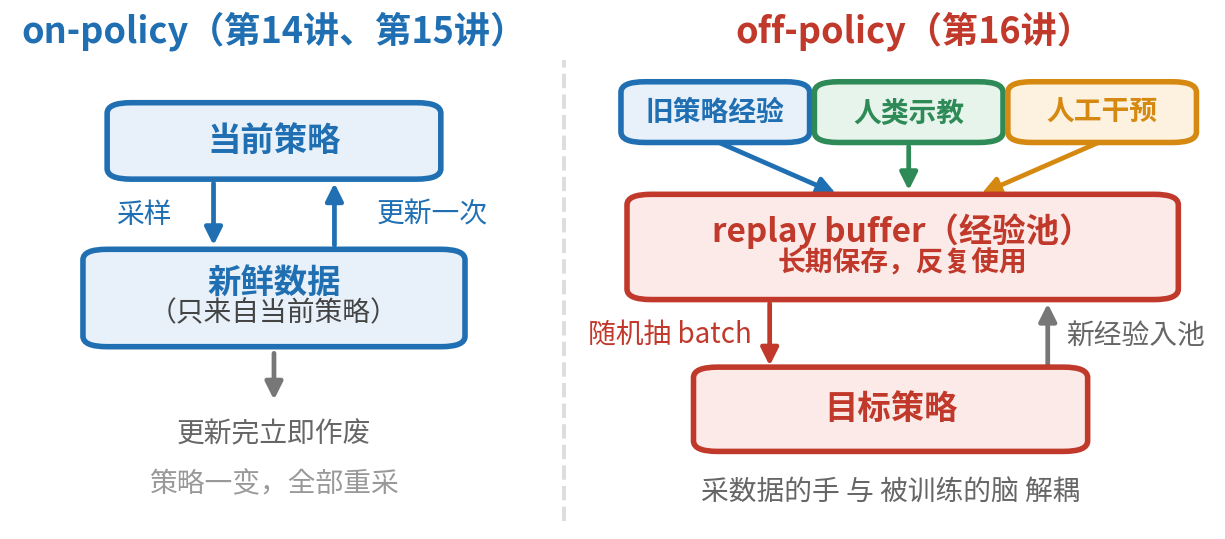
\includegraphics[width=1\linewidth,height=\textheight,keepaspectratio]{../../assets/figures/lecture14/ref/fig-onoff-dataflow.png}

}

\caption{on-policy 与 off-policy
的数据流对比：左侧数据只来自当前策略、用一次即弃；右侧多来源经验汇入经验池、长期反复使用}

\end{figure}%

两边的差别，落到图上就是\textbf{中间那个池子}：左半的数据在''当前策略''和''新鲜数据''之间打转，更新一次就作废；右半的旧策略经验、人类示教、人工干预三种来源全部汇进经验池，目标策略从池里随机抽一批训练，新经验只是继续入池。有了这个池子，数据才从消耗品变成资产------这正是第16讲上真机时必须换到
off-policy 的原因。

这个划分直接对应一笔经济账：\textbf{数据便宜（仿真随便跑）就用 on-policy
图个稳；数据贵（真机一条都不舍得扔）就用 off-policy
把经验池榨干。}本讲在仿真里训练，走 on-policy；第16讲上真机，就会换到
off-policy。

\begin{quote}
备注：\textbf{经典的似然比策略梯度}（REINFORCE、A2C、PPO 这一路）常用
on-policy
估计------因为那个梯度公式里的期望要在\textbf{当前策略}的数据分布下估；Q-learning
一族几乎总是
off-policy------因为贝尔曼最优更新跟数据是谁采的无关。但别把它读成''策略梯度必然
on-policy''：\textbf{确定性策略梯度（DDPG、TD3）和 SAC
都是用策略梯度更新 actor 的 off-policy
actor-critic}，它们从回放池里学（本节开头那张分类地图里就有这几个）。所以''基于策略
\(\approx\) on-policy、基于价值 \(\approx\)
off-policy''是\textbf{常见对应，不是定义}：两条轴一个说''学什么''、一个说''数据怎么用''，概念上独立。分不清这两条轴，是强化学习分类看着混乱的最大根源。
\end{quote}

\subsection{3.5
把算法放上地图}\label{ux628aux7b97ux6cd5ux653eux4e0aux5730ux56fe}

三个划分立好，把本讲和后面两讲会遇到的算法全部放上去：

\begin{center}
\begin{tabular}{@{}>{\raggedright\arraybackslash}p{\dimexpr 0.2090\linewidth - 2\tabcolsep\relax} >{\raggedright\arraybackslash}p{\dimexpr 0.4039\linewidth - 2\tabcolsep\relax} >{\raggedright\arraybackslash}p{\dimexpr 0.1668\linewidth - 2\tabcolsep\relax} >{\raggedright\arraybackslash}p{\dimexpr 0.2202\linewidth - 2\tabcolsep\relax}@{}}
\toprule\noalign{}
算法 & 学什么 & 数据 & 在课程里的位置 \\
\midrule\noalign{}
REINFORCE & 基于策略（策略梯度） & on-policy & 第14讲 4.3；代码 4.5（v1） \\
A2C & 基于策略（策略梯度 + critic 参照） & on-policy & 第14讲 5.3；代码 5.4（v2） \\
TRPO & 基于策略（策略梯度 + 硬约束步长） & on-policy & 第14讲 6.1（一句话带过） \\
\textbf{PPO} & 基于策略（策略梯度 + clip） & on-policy & 第14讲 6.2；代码 6.4（v3） \\
GRPO & 基于策略（策略梯度，去掉 critic，用组内平均当参照） & on-policy & 第15讲 1.4 \\
Q-learning / DQN & 基于价值 & off-policy & 第16讲 2.3--2.4 \\
SAC（及 DDPG/TD3） & 两族之间的 actor-critic & off-policy & 第16讲 5.2 \\
\bottomrule\noalign{}
\end{tabular}
\end{center}

看这张表要抓两条线：

\begin{itemize}
\tightlist
\item
  \textbf{本讲的三级阶梯 REINFORCE → A2C → PPO
  是同一支内的演进}，不是三个门类：都是
  model-free、基于策略（策略梯度）、on-policy，坐标完全相同，差别只在''怎么把策略梯度算得更稳''------这正是第
  4 节到第 6 节一节补一块的机制。演进链再往后一站就是第15讲的
  GRPO：它保留 PPO 的 clip、去掉
  critic，是这条链在大模型后训练场景下的延伸。
\item
  \textbf{第16讲换的不是''更好的算法''，而是另一格坐标}：真机数据贵，必须
  off-policy，于是从基于策略一支跳到 SAC
  那一格。到时候你会发现本讲的概念一个都不浪费。
\end{itemize}

\subsection{3.6 本节小结}\label{ux672cux8282ux5c0fux7ed3-1}

强化学习方法分类只需要三个独立的问题：学不学环境模型（model-free /
model-based）、学什么（基于价值 /
基于策略，策略梯度是基于策略的主流子类）、学的策略和采数据的策略是否同一个（on-policy
/ off-policy）。Actor-Critic 是横跨两类的\textbf{架构}词。``基于策略
\(\approx\) on-policy''只是常态对应、不是定义。本讲路线：model-free +
基于策略（策略梯度）+ on-policy，沿 REINFORCE → A2C → PPO
走到底；GRPO（第15讲）和 SAC（第16讲）都能在这张地图上找到自己的格子。

\section{4
REINFORCE：最朴素的策略梯度方法}\label{reinforceux6700ux6734ux7d20ux7684ux7b56ux7565ux68afux5ea6ux65b9ux6cd5}

\subsection{4.1
什么是策略梯度}\label{ux4ec0ux4e48ux662fux7b56ux7565ux68afux5ea6}

基于策略的方法只做一件事：调策略参数
\(\theta\)，让期望回报变大。把''期望回报''记作目标函数
\(J(\theta)\)，最直接的做法就是对它做梯度上升。\textbf{策略梯度定理}给出了这个梯度可以怎么从采样数据里估出来（结论直接用，不推导）：

\[
\nabla_\theta J(\theta)\;=\;\mathbb{E}\Big[\,\sum_t \nabla_\theta \log \pi_\theta(a_t\mid s_t)\cdot R_t\,\Big]
\]

\begin{center}
\begin{tabular}{@{}>{\raggedright\arraybackslash}p{\dimexpr 0.1724\linewidth - 2\tabcolsep\relax} >{\raggedright\arraybackslash}p{\dimexpr 0.1683\linewidth - 2\tabcolsep\relax} >{\raggedright\arraybackslash}p{\dimexpr 0.6594\linewidth - 2\tabcolsep\relax}@{}}
\toprule\noalign{}
符号 & 含义 & 说明 \\
\midrule\noalign{}
\(J(\theta)\) & 目标函数 & 当前策略的期望回报，越大越好 \\
\(\log \pi_\theta(a_t\mid s_t)\) & 对数概率 & 策略当时有多倾向于选这个动作（取对数便于求梯度） \\
\(\nabla_\theta \log \pi_\theta\) & 对数概率的梯度 & 指向''让这个动作概率变大''的参数方向 \\
\(R_t\) & 从 \(t\) 起的折扣回报 & 就是 2.3 节那个回报，在这里当这一步的''权重''（下一小节会给它一个更贴切的名字） \\
\bottomrule\noalign{}
\end{tabular}
\end{center}

沿这个梯度做上升的算法，统称\textbf{策略梯度方法}------就是 3.2
节点过名、本讲从头走到尾的那条子类链。

\subsection{4.2
梯度往哪指：好动作加概率，坏动作减概率}\label{ux68afux5ea6ux5f80ux54eaux6307ux597dux52a8ux4f5cux52a0ux6982ux7387ux574fux52a8ux4f5cux51cfux6982ux7387}

公式里两个因子各管一件事。\(\nabla_\theta \log \pi_\theta(a_t\mid s_t)\)
管方向------它指向''让动作 \(a_t\) 的概率变大''；乘上去的权重 \(R_t\)
管力度：

\begin{itemize}
\tightlist
\item
  \(R_t\)
  大（这一步之后拿了高回报）：往''更常做这个动作''的方向推得狠一点；
\item
  \(R_t\) 小甚至为负：反着推，让它以后少出现。
\end{itemize}

\begin{quote}
好动作提高概率，坏动作降低概率------按事后的回报大小定推拉的力度。
\end{quote}

权重用的是 \textbf{reward-to-go}（\(t\)
之后的回报）而不是整条轨迹的总回报，道理也直白：评价 \(t\)
时刻的动作，只该算它\textbf{之后}的账；它之前已经发生的奖励与这个动作无关，混进来只添噪声。

落成损失函数，就是在前面加个负号交给梯度下降。下面这一行等会儿会原样出现在
v1 的代码里（代码里那个 \texttt{advantages} 目前就是 \(R_t\)
做了一点归一化，4.5 节细说）：

\begin{Shaded}
\begin{Highlighting}[]
\NormalTok{policy\_loss }\OperatorTok{=} \OperatorTok{{-}}\NormalTok{(log\_probs }\OperatorTok{*}\NormalTok{ batch[}\StringTok{"advantages"}\NormalTok{]).mean()}
\end{Highlighting}
\end{Shaded}

\subsection{4.3
REINFORCE：采一批轨迹、算回报、更新一次}\label{reinforceux91c7ux4e00ux6279ux8f68ux8ff9ux7b97ux56deux62a5ux66f4ux65b0ux4e00ux6b21}

把上面的公式变成可执行的循环，就是
REINFORCE，教材上也叫\textbf{蒙特卡洛策略梯度}{[}5{]}------``蒙特卡洛''指权重
\(R_t\) 是用\textbf{实际跑出来的回报}直接估的，不借助任何辅助网络：

\begin{enumerate}
\def\labelenumi{\arabic{enumi}.}
\tightlist
\item
  用当前策略在环境里采一批轨迹；
\item
  对每一步算 reward-to-go \(R_t\)；
\item
  按 \(-\log\pi_\theta(a_t\mid s_t)\cdot R_t\) 更新一次策略；
\item
  \textbf{丢掉这批数据}（on-policy：策略变了，旧数据即过期），回到第 1
  步。
\end{enumerate}

这是所有策略梯度算法的公共骨架。后面的 A2C 和 PPO
都只是在这四步里''换零件''：A2C 换第 2 步的权重，PPO 改第 3
步的更新方式。

\subsection{4.4 认识三个外部依赖：mjlab、GVHMR 与
GMR}\label{ux8ba4ux8bc6ux4e09ux4e2aux5916ux90e8ux4f9dux8d56mjlabgvhmr-ux4e0e-gmr}

跑实验之前，先认识几位''幕后工作人员''。下一节代码走读里的
\texttt{code/rl/1\_rl\_basics/1\_1\_g1\_walk\_rl/env.py}
只是薄薄一层包装，真正干重活的是几个开源组件。它们是本讲实验的依赖，不是研究对象------每一位用一段话知道它是谁、替我们干了什么，就足够了。

第一位是 \textbf{mjlab}{[}7{]}，G1
的''练功房''。强化学习靠海量试错吃饭，一个环境一步一步跑太慢，我们的训练一次开
4096 个环境同时采样。mjlab 把 GPU 并行版的 MuJoCo（MuJoCo Warp）接进
Isaac Lab
那套按管理器组装环境的接口：场景、观测、奖励、终止条件都是现成积木，还内置了宇树
G1
的标准任务------行走实验用的平地速度跟随（\texttt{Mjlab-Velocity-Flat-Unitree-G1}）、6.6
节动作跟随用的动作跟踪（\texttt{Mjlab-Tracking-Flat-Unitree-G1}），都直接取自它。课程这层包装做的只是把它的接口整理得顺手一点。

\begin{figure}[H]

{\centering 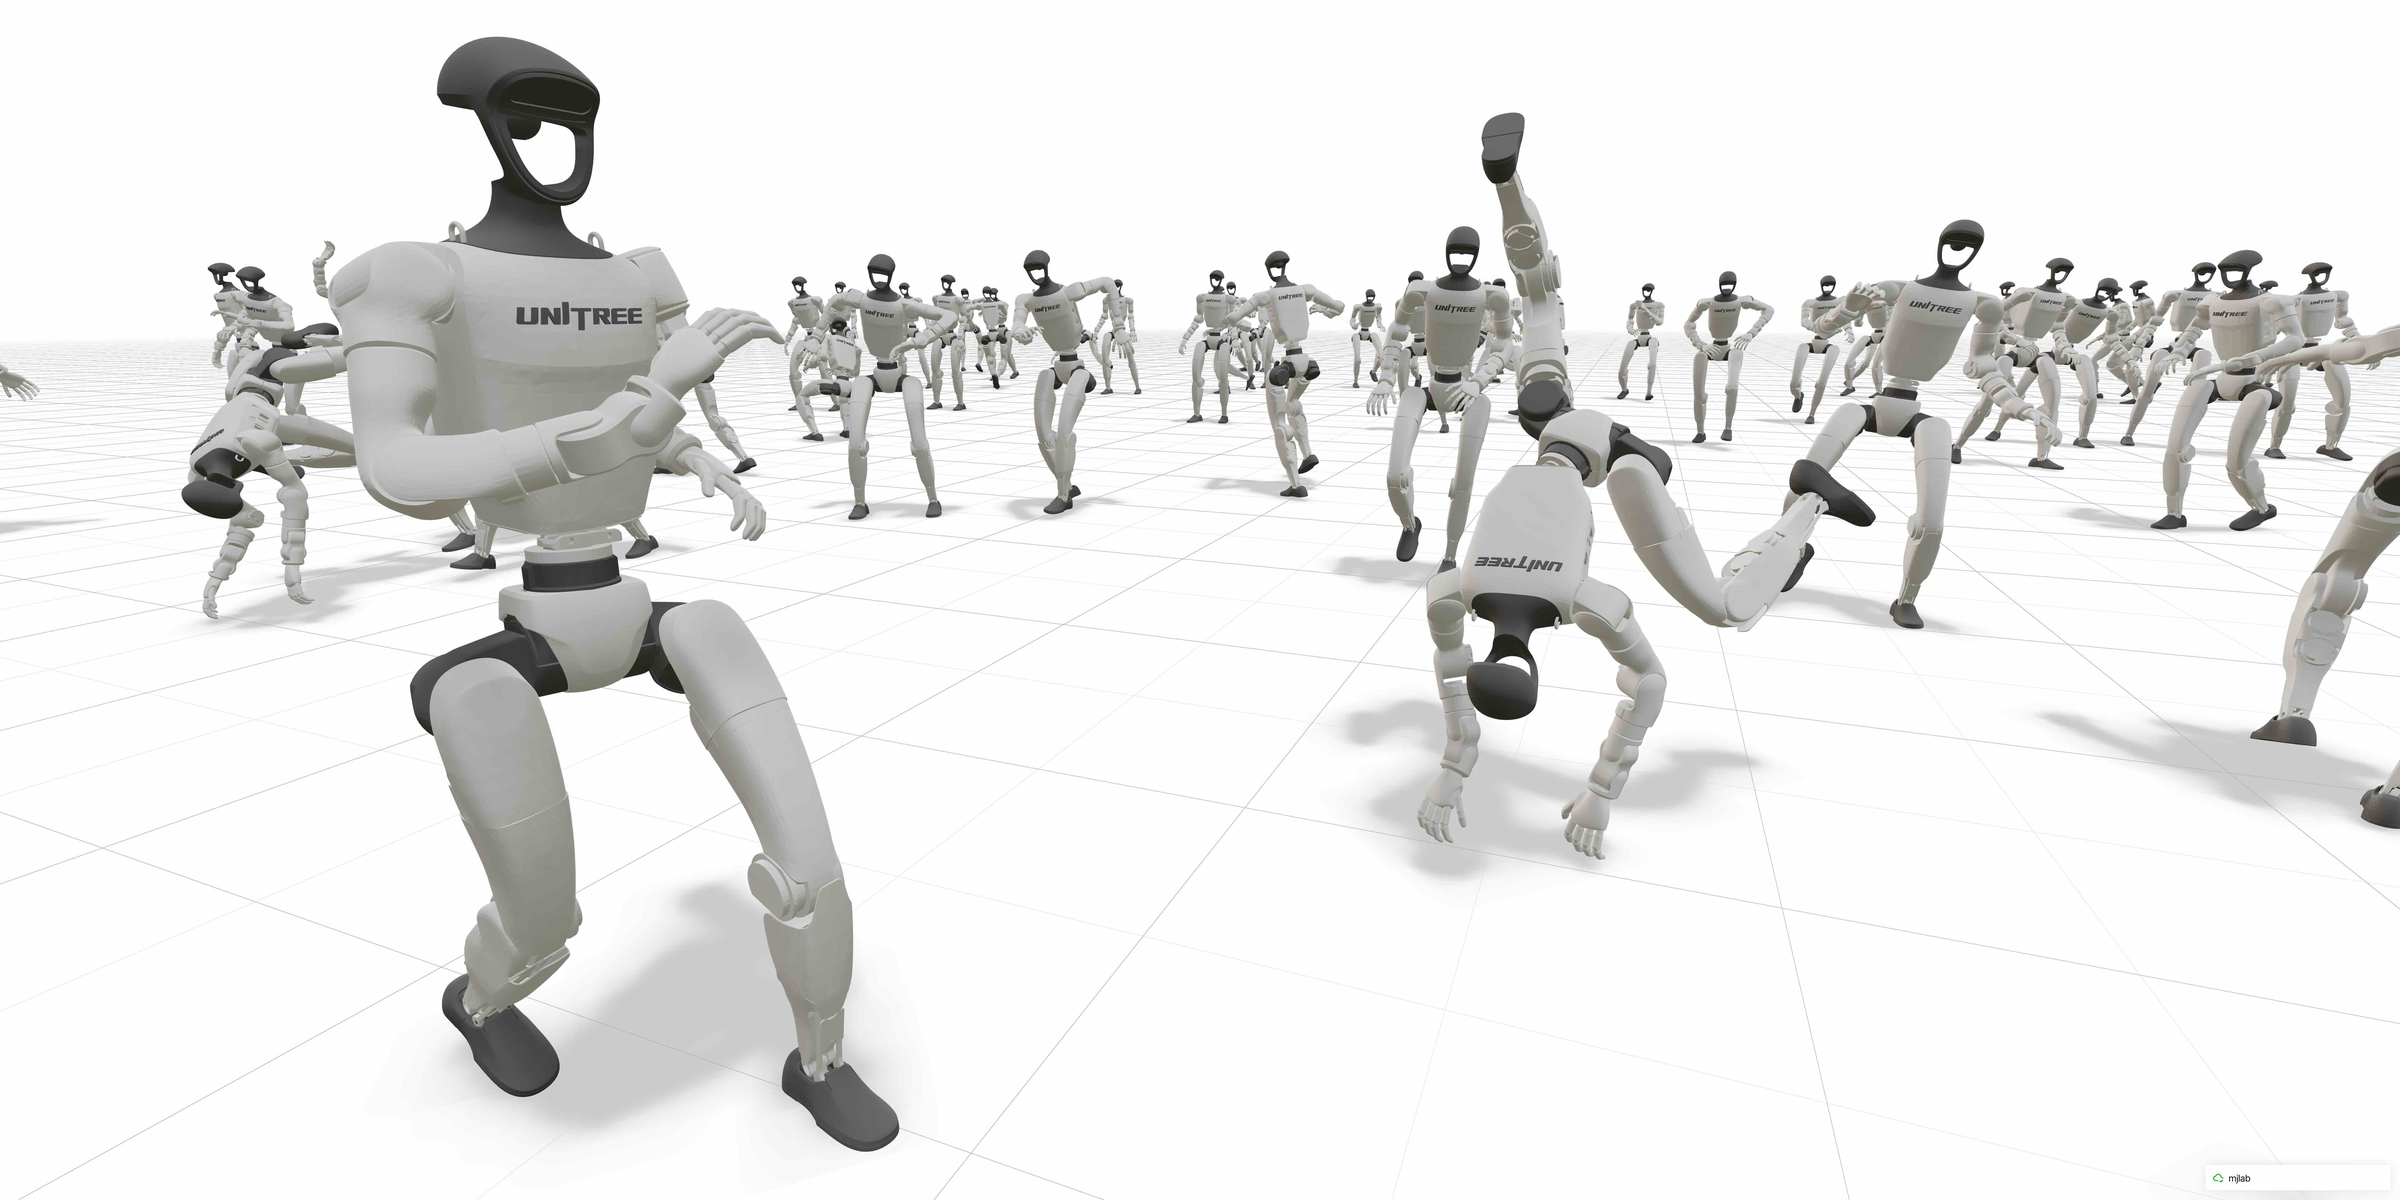
\includegraphics[width=0.92\linewidth,height=\textheight,keepaspectratio]{../../assets/figures/lecture14/ref/fig145-mjlab-parallel.png}

}

\caption{mjlab 并行仿真中的大批宇树
G1，同屏各自执行行走、翻滚等不同动作，GPU
并行让''海量试错''在一张显卡上成为可能。图出自 mjlab 项目主页（右下角带
mjlab 水印），见参考文献 7}

\end{figure}%

第二位是 \textbf{GVHMR}{[}8{]}，负责从视频里''抠''出人的动作。6.6 节要让
G1
逐帧贴住一段真实武术动作，参考动作最方便的来源是一段普通视频。GVHMR（浙江大学团队开源）输入单目视频，输出世界坐标系下连贯的三维人体动作------人在哪里、朝向哪边、每一帧什么姿势，全部恢复出来，并用
SMPL-X
参数化人体表示（用一组低维参数描述体型与逐帧姿态，相当于人体动作的通用''语言''）。它的做法是先把姿态估计在一个由\textbf{重力方向
+
相机朝向}定义的坐标系里，再靠相机旋转转回世界系，从而避开''世界坐标系怎么定''这个老问题。

\begin{figure}[H]

{\centering 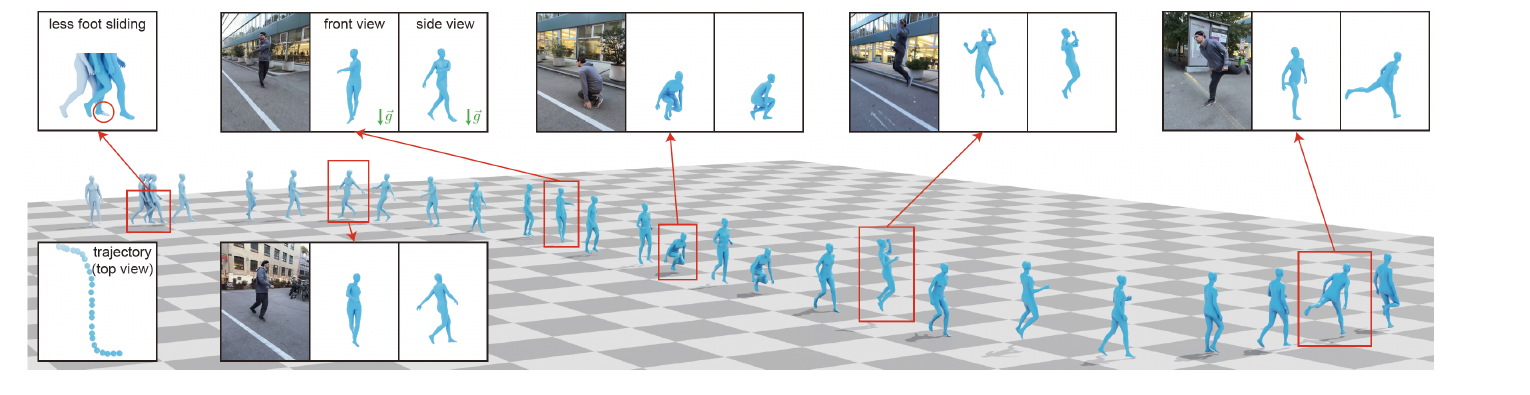
\includegraphics[width=0.98\linewidth,height=\textheight,keepaspectratio]{../../assets/figures/lecture14/ref/fig145-gvhmr-teaser_arxiv-2409.06662.png}

}

\caption{GVHMR
从街头单目视频恢复世界坐标系下的人体动作：蓝色人体网格为恢复结果，沿真实运动轨迹排开；四周小图给出若干帧的原始画面与恢复姿态的正、侧视对照（绿色箭头是重力方向），左上角与左下角两块分别展示脚部打滑更少、以及俯视的运动轨迹。图出自参考文献
8}

\end{figure}%

第三位是 \textbf{GMR}（General Motion
Retargeting）{[}9{]}{[}10{]}，负责把''人的动作''翻译成''G1
的动作''。人和 G1
体型比例不同、关节构成也不同，人的动作不能直接照搬到机器人身上；这道翻译工序的术语叫\textbf{重定向}（retargeting）。GMR
先对齐人与机器人的关键部位、按体型做缩放，再用逆运动学逐帧解出 G1
各关节的角度，输出机器人真正能执行的参考轨迹。

\begin{figure}[H]

{\centering 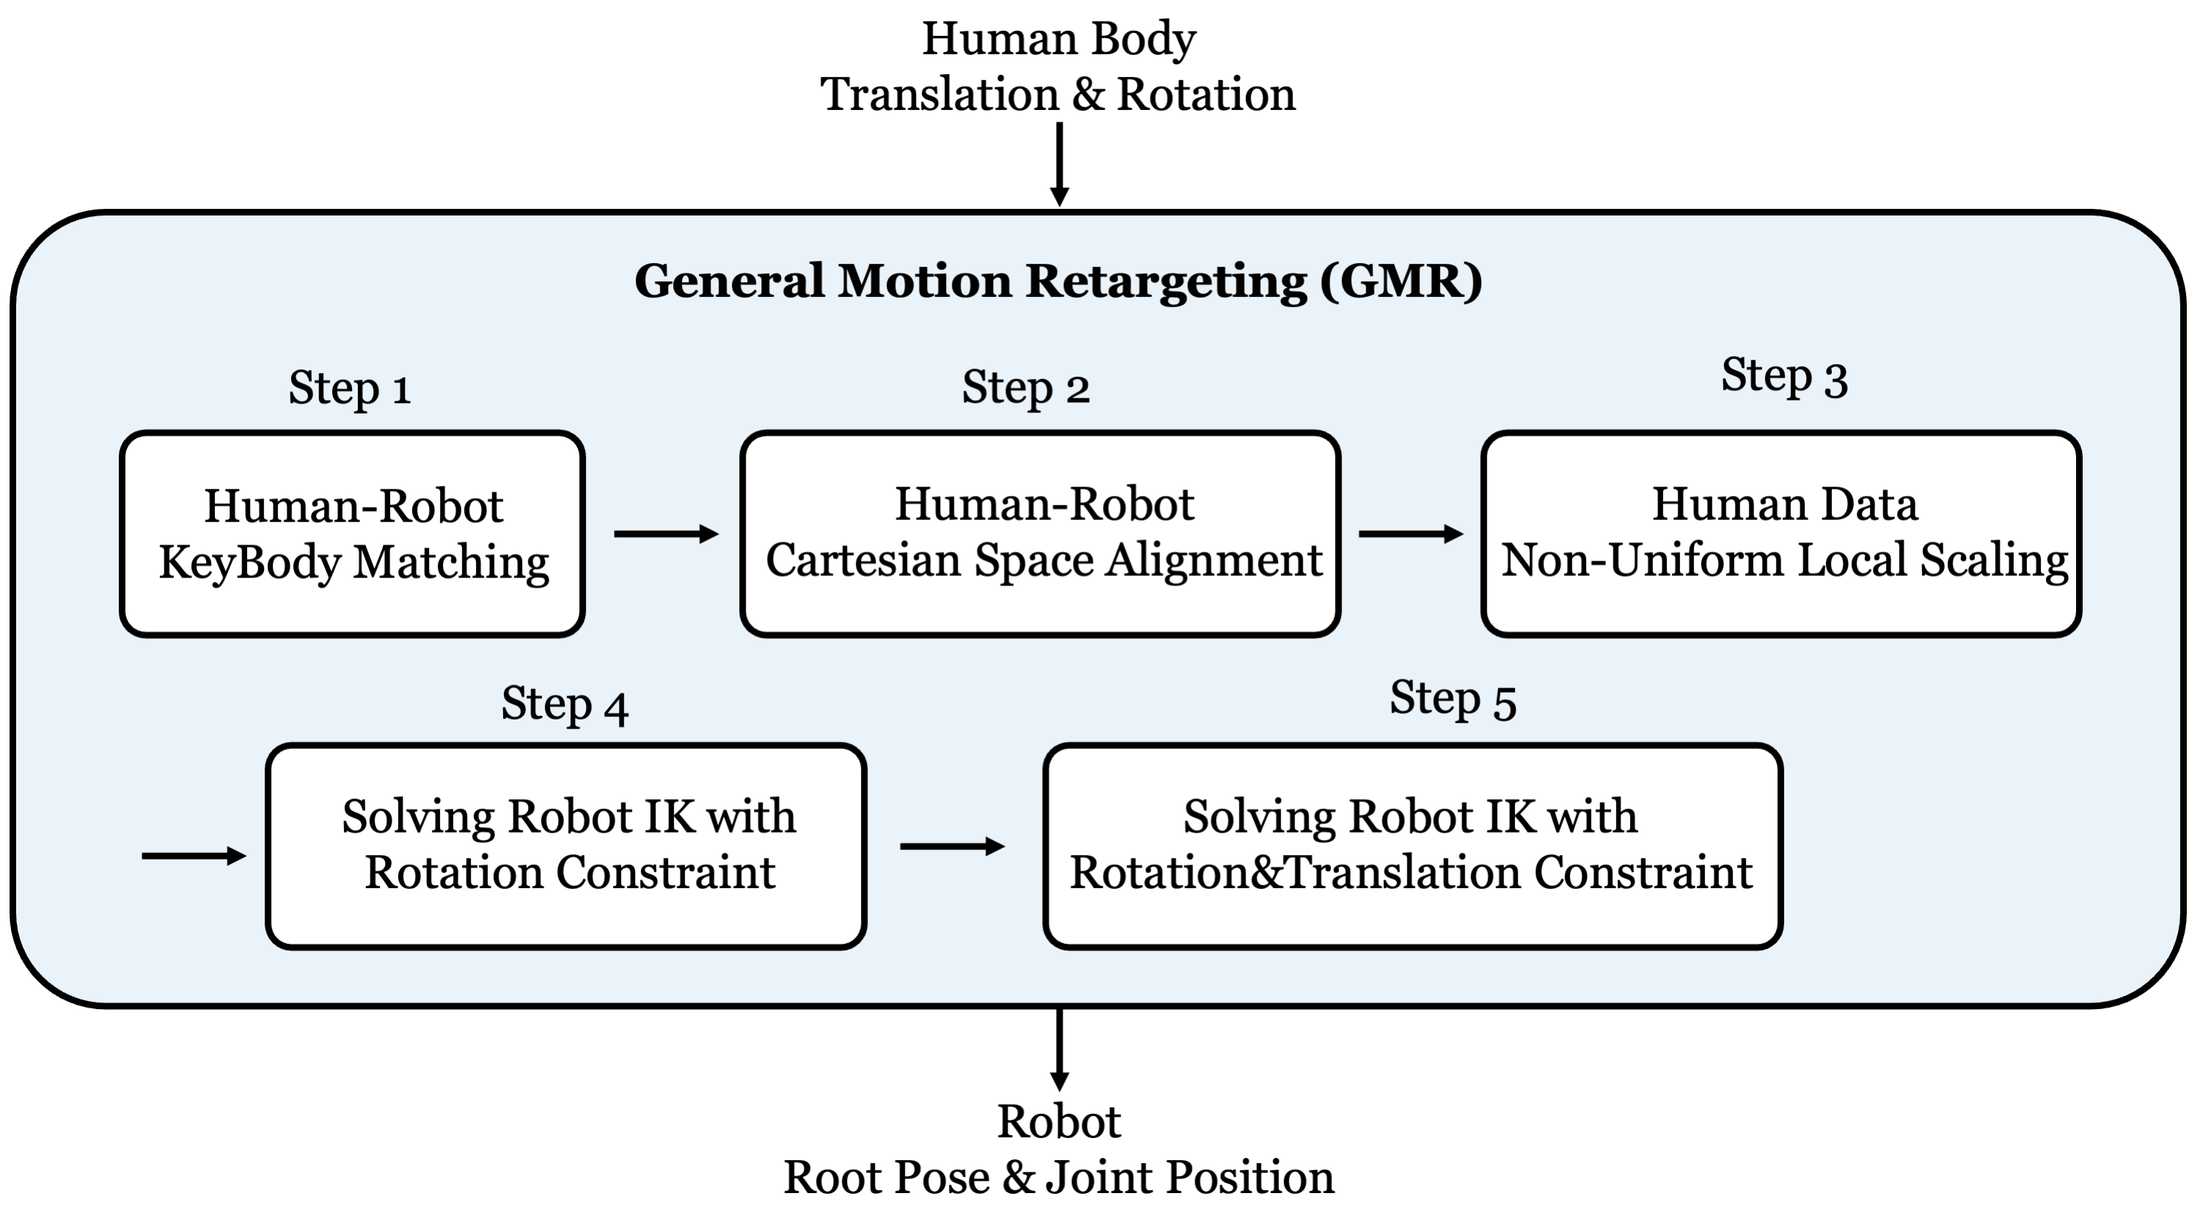
\includegraphics[width=0.8\linewidth,height=\textheight,keepaspectratio]{../../assets/figures/lecture14/ref/fig145-gmr-pipeline_arxiv-2510.02252.png}

}

\caption{GMR
的重定向流程：输入人体各部位的平移与旋转，经关键部位匹配、笛卡尔空间对齐、非均匀局部缩放，再两轮求解带约束的机器人逆运动学，输出机器人根姿态与关节位置。图出自参考文献
9}

\end{figure}%

从一段视频开始，先用 GVHMR 恢复人体动作，再用 GMR 重定向成 G1
参考动作------这条预处理管线在课程实验仓库里是独立模块
\texttt{code/rl/1\_rl\_basics/1\_2\_video\_to\_g1\_reference/}，产物是一个参考动作文件
\texttt{code/rl/1\_rl\_basics/data/g1\_reference\_motions/marshal-arts.npz}（682
帧、50 Hz、29 个关节）。本讲的行走实验只用到 mjlab；这份参考动作，等 6.6
节动作跟随登场时才派上用场。

\subsection{4.5 代码走读：v1
版训练循环}\label{ux4ee3ux7801ux8d70ux8bfbv1-ux7248ux8badux7ec3ux5faaux73af}

行走实验的代码都在 \texttt{code/rl/1\_rl\_basics/1\_1\_g1\_walk\_rl/}
这一个目录里。本节走读前三个文件，其中前两个由三个版本共用；后三个不讲算法，但
4.6 节起的评测数字、rollout 视频和 6.5
节那两张训练曲线图，都由它们产出：

\begin{center}
\begin{tabular}{@{}>{\raggedright\arraybackslash}p{\dimexpr 0.4500\linewidth - 2\tabcolsep\relax} >{\raggedright\arraybackslash}p{\dimexpr 0.5500\linewidth - 2\tabcolsep\relax}@{}}
\toprule\noalign{}
文件 & 职责 \\
\midrule\noalign{}
\texttt{code/rl/1\_\allowbreak rl\_\allowbreak basics/1\_\allowbreak 1\_\allowbreak g1\_\allowbreak walk\_\allowbreak rl/env.py} & 包装 mjlab 的 G1 平地速度任务成 \texttt{G1WalkEnv}，返回观测 / 奖励 / 终止信号 \\
\texttt{code/rl/1\_\allowbreak rl\_\allowbreak basics/1\_\allowbreak 1\_\allowbreak g1\_\allowbreak walk\_\allowbreak rl/model.py} & \texttt{ActorCritic} 网络（actor + critic 两个 MLP）与 GAE 工具函数 \\
\texttt{code/rl/1\_\allowbreak rl\_\allowbreak basics/1\_\allowbreak 1\_\allowbreak g1\_\allowbreak walk\_\allowbreak rl/train\_\allowbreak v1\_\allowbreak reinforce.py} & 本节的 REINFORCE 训练脚本 \\
\texttt{code/rl/1\_\allowbreak rl\_\allowbreak basics/1\_\allowbreak 1\_\allowbreak g1\_\allowbreak walk\_\allowbreak rl/rollout.py} & 载入训练好的权重，按 1.4 节的统一口径（16 个环境 × 400 步、确定性动作）评测并录像 \\
\texttt{code/rl/1\_\allowbreak rl\_\allowbreak basics/1\_\allowbreak 1\_\allowbreak g1\_\allowbreak walk\_\allowbreak rl/plot\_\allowbreak reward\_\allowbreak curves.py} & 画 6.5 节那张三算法训练奖励对照曲线 \\
\texttt{code/rl/1\_\allowbreak rl\_\allowbreak basics/1\_\allowbreak 1\_\allowbreak g1\_\allowbreak walk\_\allowbreak rl/plot\_\allowbreak training\_\allowbreak losses.py} & 画 6.5 节那张四面板训练损失对照图 \\
\bottomrule\noalign{}
\end{tabular}
\end{center}

评测摘要落在 \texttt{code/rl/1\_rl\_basics/result/1\_1\_g1\_walk\_rl/}
下的同名 \texttt{.json}
里，后面每一个奖励与摔倒率都能在那里查到原始记录。

Lightning 把训练拆成三块（第12讲 4.6 节见过 \texttt{LightningModule} 与
\texttt{LightningDataModule}
的这套分工）；唯一不同的是这里的''数据集''不再是磁盘上的文件，而是\textbf{在线采样}：

\begin{center}
\begin{tabular}{@{}>{\raggedright\arraybackslash}p{\dimexpr 0.3823\linewidth - 2\tabcolsep\relax} >{\raggedright\arraybackslash}p{\dimexpr 0.6177\linewidth - 2\tabcolsep\relax}@{}}
\toprule\noalign{}
类 & 角色 \\
\midrule\noalign{}
\texttt{G1WalkRolloutDataset} & 在线数据集：每轮用当前策略采一段轨迹，产出一整批（batch）训练数据 \\
\texttt{G1WalkData} & \texttt{LightningDataModule}：每一轮（Lightning 管一轮叫一个 epoch）都重建数据集，保证数据永远新鲜，对应 on-policy \\
\texttt{G1WalkLightningReinforce} & \texttt{LightningModule}：拿到 batch 算 REINFORCE loss \\
\bottomrule\noalign{}
\end{tabular}
\end{center}

采样端的核心是 reward-to-go
的计算------从后往前累加折扣回报，遇到回合结束就截断：

\begin{Shaded}
\begin{Highlighting}[]
\KeywordTok{def}\NormalTok{ reward\_to\_go(reward\_steps, done\_steps, gamma):}
\NormalTok{    returns }\OperatorTok{=}\NormalTok{ torch.zeros\_like(reward\_steps)}
\NormalTok{    running }\OperatorTok{=}\NormalTok{ torch.zeros(reward\_steps.shape[}\DecValTok{1}\NormalTok{], device}\OperatorTok{=}\NormalTok{reward\_steps.device)}
    \ControlFlowTok{for}\NormalTok{ step }\KeywordTok{in} \BuiltInTok{reversed}\NormalTok{(}\BuiltInTok{range}\NormalTok{(reward\_steps.shape[}\DecValTok{0}\NormalTok{])):}
\NormalTok{        running }\OperatorTok{=}\NormalTok{ reward\_steps[step] }\OperatorTok{+}\NormalTok{ gamma }\OperatorTok{*}\NormalTok{ running }\OperatorTok{*}\NormalTok{ (}\FloatTok{1.0} \OperatorTok{{-}}\NormalTok{ done\_steps[step])}
\NormalTok{        returns[step] }\OperatorTok{=}\NormalTok{ running}
    \ControlFlowTok{return}\NormalTok{ returns}
\end{Highlighting}
\end{Shaded}

采完 4096 环境 × 24 步的一段轨迹后，把回报整理成每步的权重：

\begin{Shaded}
\begin{Highlighting}[]
\NormalTok{        returns }\OperatorTok{=}\NormalTok{ reward\_to\_go(reward\_steps, done\_steps, }\VariableTok{self}\NormalTok{.gamma)}
        \CommentTok{\# 唯一的基线就是整批均值（常数），没有学习的 critic。}
\NormalTok{        advantages }\OperatorTok{=}\NormalTok{ returns }\OperatorTok{{-}}\NormalTok{ returns.mean()}
\NormalTok{        advantages }\OperatorTok{=}\NormalTok{ advantages }\OperatorTok{/}\NormalTok{ (advantages.std() }\OperatorTok{+} \FloatTok{1.0e{-}8}\NormalTok{)}
\end{Highlighting}
\end{Shaded}

这里有个值得停一秒的小动作：权重没有直接用
\(R_t\)，而是先\textbf{减掉整批均值}再除以整批标准差。这是常见的方差降低与尺度归一化技巧，让数值更平稳。要说准确一点：\(b(s)\)
那条''减去与动作无关的基线不改变梯度期望''的性质，要求基线是\textbf{固定的、不依赖当前所选动作的}；而这里的批均值恰恰是用同一批的动作和回报算出来的，除以批标准差也会引入有限样本偏差。所以它不是严格无偏，只是在实践里以一点小偏差换取稳定性------好用，但别说成''完全不改变梯度期望''。而''跟平均水平比，而不是跟零比''这个念头，正是下一节整节的种子，先按下不表。

训练端的 \texttt{training\_step} 就是 4.2 节那行公式，外加一项熵：

\begin{Shaded}
\begin{Highlighting}[]
    \KeywordTok{def}\NormalTok{ training\_step(}\VariableTok{self}\NormalTok{, batch, batch\_idx):}
\NormalTok{        distribution }\OperatorTok{=} \VariableTok{self}\NormalTok{.model.action\_distribution(batch[}\StringTok{"obs"}\NormalTok{])}
\NormalTok{        log\_probs }\OperatorTok{=}\NormalTok{ distribution.log\_prob(batch[}\StringTok{"actions"}\NormalTok{]).}\BuiltInTok{sum}\NormalTok{(dim}\OperatorTok{={-}}\DecValTok{1}\NormalTok{)}
\NormalTok{        entropy }\OperatorTok{=}\NormalTok{ distribution.entropy().}\BuiltInTok{sum}\NormalTok{(dim}\OperatorTok{={-}}\DecValTok{1}\NormalTok{)}
\NormalTok{        policy\_loss }\OperatorTok{=} \OperatorTok{{-}}\NormalTok{(log\_probs }\OperatorTok{*}\NormalTok{ batch[}\StringTok{"advantages"}\NormalTok{]).mean()}
\NormalTok{        entropy\_loss }\OperatorTok{=}\NormalTok{ entropy.mean()}
\NormalTok{        loss }\OperatorTok{=}\NormalTok{ policy\_loss }\OperatorTok{{-}} \VariableTok{self}\NormalTok{.entropy\_coef }\OperatorTok{*}\NormalTok{ entropy\_loss}
\end{Highlighting}
\end{Shaded}

多出来的\textbf{熵奖励}（\texttt{entropy\_coef\ =\ 0.01}）鼓励动作分布别过早收窄------分布越''摊开''熵越大，等于奖励策略保持探索。这就是
2.4
节说的''随机性是探索的来源''在代码里的落点；三个版本都带这一项，它不是版本间的区别点。

还有一处点破：\texttt{ActorCritic} 网络里其实有 critic，但 v1
的优化器\textbf{刻意只训 actor}------

\begin{Shaded}
\begin{Highlighting}[]
    \KeywordTok{def}\NormalTok{ configure\_optimizers(}\VariableTok{self}\NormalTok{):}
        \CommentTok{\# 只优化 actor 和动作标准差；critic 不参与训练。}
\NormalTok{        params }\OperatorTok{=} \BuiltInTok{list}\NormalTok{(}\VariableTok{self}\NormalTok{.model.actor.parameters()) }\OperatorTok{+}\NormalTok{ [}\VariableTok{self}\NormalTok{.model.std]}
        \VariableTok{self}\NormalTok{.optimizer }\OperatorTok{=}\NormalTok{ torch.optim.Adam(params, lr}\OperatorTok{=}\VariableTok{self}\NormalTok{.learning\_rate)}
        \ControlFlowTok{return} \VariableTok{self}\NormalTok{.optimizer}
\end{Highlighting}
\end{Shaded}

这是为了三版共用同一个网络类、保证对照干净：v1 的 critic
纯粹闲置，REINFORCE 本身完全不需要它。入口照例是
\texttt{trainer.fit(model,\ data)}，其中
\texttt{reload\_dataloaders\_every\_n\_epochs=1}
让每轮都重新采样------on-policy 的''用完即弃''由 Lightning
的数据加载周期天然实现。

\subsection{4.6 实验：G1 用 REINFORCE
学走路}\label{ux5b9eux9a8cg1-ux7528-reinforce-ux5b66ux8d70ux8def}

按 1.4 节的统一口径评测（最终权重、确定性动作、16 环境 × 400 步）：

\begin{center}
\begin{tabular}{@{}>{\raggedright\arraybackslash}p{\dimexpr 0.2188\linewidth - 2\tabcolsep\relax} >{\raggedright\arraybackslash}p{\dimexpr 0.2188\linewidth - 2\tabcolsep\relax}@{}}
\toprule\noalign{}
指标 & v1 REINFORCE \\
\midrule\noalign{}
评测平均奖励 & 0.070 \\
摔倒率 & 1.3\% \\
\bottomrule\noalign{}
\end{tabular}
\end{center}

\begin{figure}[H]

{\centering 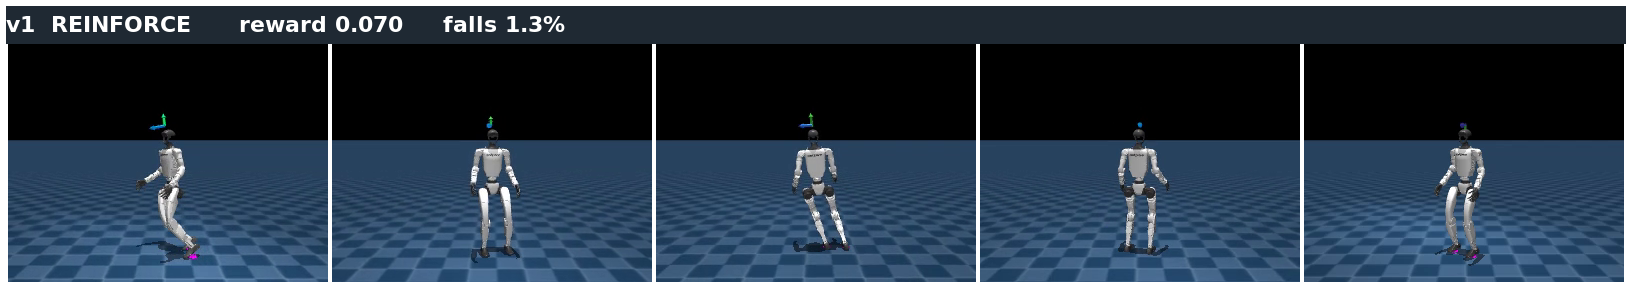
\includegraphics[width=0.98\linewidth,height=\textheight,keepaspectratio]{../../assets/figures/lecture14/ref/fig146-walk-v1.png}

}

\caption{v1 REINFORCE 训练 3000 迭代后的 rollout
关键帧，从左到右为同一段时间内的连续时刻：G1
能保持站立并小幅挪步，但姿态僵硬、动作幅度小，偶有摔倒}

\end{figure}%

先说成绩：\textbf{它真的学会了}。从随机初始化出发------最初的策略只会让
G1
像断线木偶一样瘫倒------训练之后能站住、能顺着指令小幅挪步。这说明''好动作加概率、坏动作减概率''这个信号是实打实起作用的，策略梯度这条路走得通。

再说不足，看图和数字都很明显：动作僵硬、不敢迈步，跟指令跟得很勉强，还有
1.3\% 的评测回合以摔倒收场。训练过程也不好看------奖励爬到 700
次迭代左右就停在 0.008 附近，剩下的两千多次迭代基本原地踏步（6.5
节那张训练曲线看得最清楚）。能学，但学得\textbf{又慢又浅}。

\subsection{4.7
毛病在哪：回报噪声淹没了学习信号}\label{ux6bdbux75c5ux5728ux54eaux56deux62a5ux566aux58f0ux6df9ux6ca1ux4e86ux5b66ux4e60ux4fe1ux53f7}

病根在权重 \(R_t\)
上。它是蒙特卡洛估计------\textbf{这一步之后实际发生的一切}都被算进这个数里：同一个状态下做同一个好动作，这次后面一路顺风、拿了高回报；下次同样的开局，后面那几十步走岔了、摔了，回报就低。于是''这个动作好不好''的信号里，混进了大量\textbf{与这个动作无关的运气}。

这就是\textbf{高方差}：梯度的方向平均来看是对的，但每一次估计都在真值周围剧烈乱跳。4096
个环境的平均能压掉一部分，但对 29
维连续动作的人形任务远远不够------大部分更新步都在相互抵消，真正推着策略往前走的那点分量被剩下的噪声稀释掉了。

减掉整批均值那个小动作已经暗示了出路：\textbf{别拿绝对回报当权重，找个参照物，比出相对好坏}。参照物选得越贴切，运气成分抵消得越干净。什么是最贴切的参照物？下一节的主角。

\subsection{4.8 本节小结}\label{ux672cux8282ux5c0fux7ed3-2}

策略梯度方法沿''期望回报的梯度''直接更新策略，REINFORCE
是它最朴素的实现：用实际回报（reward-to-go）当权重，好动作加概率、坏动作减概率，采一批、更一步、丢数据。在
G1 行走上它证明了这条路走得通（能站能挪，0.070 / 摔
1.3\%），但蒙特卡洛回报里混着大量与动作无关的运气，\textbf{方差大}，学得又慢又浅。它的局限指向一个明确的改进方向：给回报找一个像样的参照物。

\section{5
A2C：请一位评分员来降方差}\label{a2cux8bf7ux4e00ux4f4dux8bc4ux5206ux5458ux6765ux964dux65b9ux5dee}

\subsection{5.1
基线的直觉：跟「平均水平」比，不是跟零比}\label{ux57faux7ebfux7684ux76f4ux89c9ux8ddfux5e73ux5747ux6c34ux5e73ux6bd4ux4e0dux662fux8ddfux96f6ux6bd4}

评价一个动作，公平的问法不是''它拿了多少分''，而是''它比\textbf{这个状态下的平均水平}多拿了多少分''。同样是''后面拿到回报
5''，在一个平均只能拿 1 的烂局面里是神来之笔，在平均能拿 10
的好局面里是拖了后腿。

把这个参照物记作\textbf{基线（baseline）}\(b(s)\)：策略梯度的权重从
\(R_t\) 换成 \(R_t - b(s_t)\)。数学上可以证明（这里直接引用结论）：只要
\(b\)
不依赖动作，减掉它\textbf{不改变梯度的期望}，却能大幅降低方差------运气带来的涨落被参照物同步吸收了。带基线的
REINFORCE 在教材里就叫 \textbf{REINFORCE with baseline}{[}5{]}。

v1
已经偷偷用了最粗的基线：整批回报的均值，一个常数。但常数对所有状态一视同仁，显然不够贴切------烂局面和好局面的''平均水平''根本不同。\textbf{理想的基线应该因状态而异：每个状态自己的平均水平。}这个''每个状态自己的平均水平''，正是
2.4 节预告过的那个量。

\subsection{5.2 价值函数与优势：V、Q、A = Q −
V}\label{ux4ef7ux503cux51fdux6570ux4e0eux4f18ux52bfvqa-q-v}

现在正式引入价值。先看\textbf{状态价值函数} \(V^\pi(s)\)：

\[
V^\pi(s)=\mathbb{E}_{\pi}\big[\,r_{t+1}+\gamma r_{t+2}+\gamma^2 r_{t+3}+\cdots \,\mid\, s_t=s\,\big]
\]

\(V^\pi(s)\) 回答''\textbf{这个状态本身有多好}''------从 \(s\)
出发、之后都按当前策略 \(\pi\)
走，平均能拿到多少回报。它不规定第一步做哪个动作------这正是''这个状态的平均水平''的严格说法，也就是我们要的理想基线。

再看\textbf{动作价值函数} \(Q^\pi(s,a)\)，它比 \(V\) 多指定了第一步：

\[
Q^\pi(s,a)=\mathbb{E}\big[\,r_{t+1}+\gamma r_{t+2}+\gamma^2 r_{t+3}+\cdots \,\mid\, s_t=s,\ a_t=a\,\big]
\]

即在状态 \(s\) 下\textbf{先做动作 \(a\)}、之后再按 \(\pi\)
走的平均回报（3.2
节基于价值的方法学的就是它）。两者一减，得到全场最重要的量------\textbf{优势函数（advantage）}：

\[
A^\pi(s,a)=Q^\pi(s,a)-V^\pi(s)
\]

它回答的问题正是 5.1
节那个公平的问法：\textbf{这个动作比该状态的平均水平好多少？}

\begin{itemize}
\tightlist
\item
  \(A(s,a)>0\)：比平均好，\textbf{提高}它的概率；
\item
  \(A(s,a)<0\)：比平均差，\textbf{降低}它的概率；
\item
  \(A(s,a)\approx 0\)：和平均差不多，基本不用动。
\end{itemize}

\begin{center}
\begin{tabular}{@{}>{\raggedright\arraybackslash}p{\dimexpr 0.1164\linewidth - 2\tabcolsep\relax} >{\raggedright\arraybackslash}p{\dimexpr 0.1220\linewidth - 2\tabcolsep\relax} >{\raggedright\arraybackslash}p{\dimexpr 0.7616\linewidth - 2\tabcolsep\relax}@{}}
\toprule\noalign{}
符号 & 含义 & 说明 \\
\midrule\noalign{}
\(b(s)\) & 基线 & 只依赖状态、不依赖所选动作的参照物；这类基线减掉后不改变梯度期望 \\
\(V^\pi(s)\) & 状态价值 & 状态 \(s\) 的平均水平------理想的基线 \\
\(Q^\pi(s,a)\) & 动作价值 & 在 \(s\) 先做 \(a\) 有多好 \\
\(A^\pi(s,a)\) & 优势 & \(Q-V\)，动作比平均好多少------理想的权重 \\
\bottomrule\noalign{}
\end{tabular}
\end{center}

从此策略梯度的权重升级为优势：\textbf{估出每个动作的
\(A\)，优势为正就调高概率、为负就调低。}本讲余下的一切、以及第15讲的
GRPO，全在围绕''怎么把 \(A\) 估得又准又稳''做文章。

\subsection{5.3 从基线到 critic：Actor-Critic 与
GAE}\label{ux4eceux57faux7ebfux5230-criticactor-critic-ux4e0e-gae}

\(V^\pi(s)\)
没有解析解，那就用老办法------再训一个小网络去估它，输入状态、输出一个标量。这个价值网络就是
\textbf{critic（评分员）}，原来的策略网络对应地叫
\textbf{actor（演员）}：演员出动作，评分员打分。

\begin{figure}[H]

{\centering 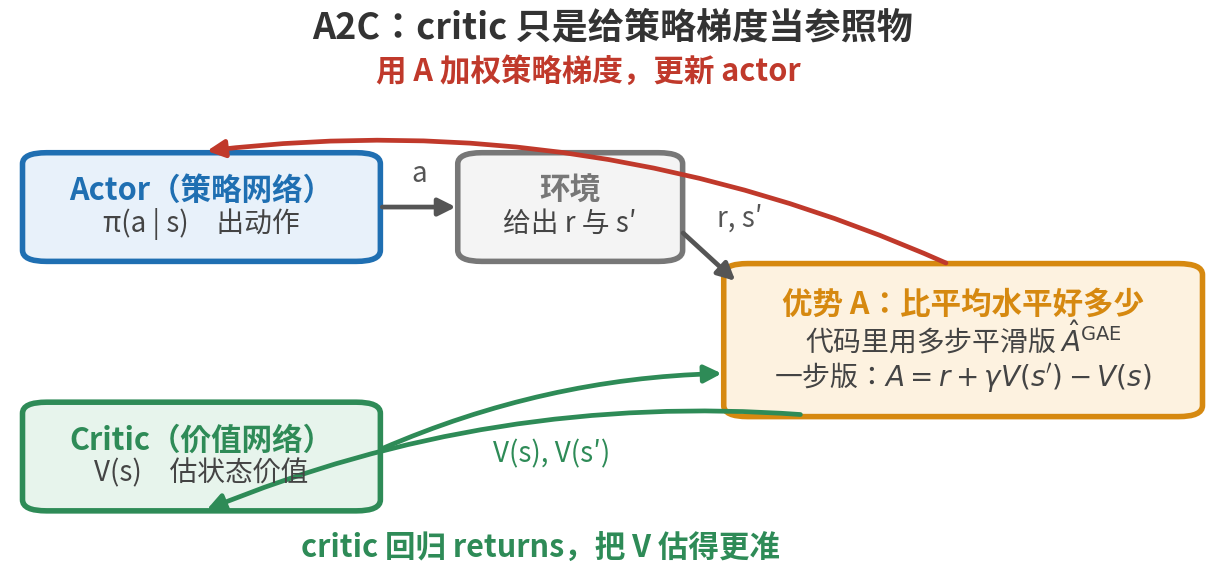
\includegraphics[width=1\linewidth,height=\textheight,keepaspectratio]{../../assets/figures/lecture14/ref/fig-actor-critic-a2c.png}

}

\caption{A2C 的 Actor-Critic
分工：actor（策略网络）出动作，critic（价值网络）估状态价值、帮 actor
算优势。优化主体仍是策略，critic 只当参照物}

\end{figure}%

顺着图上的箭头走一遍就是一轮更新：actor 出动作交给环境，环境回一个 \(r\)
和一个 \(s'\)；critic 拿状态估出
\(V(s)\)、\(V(s')\)，两路汇到右边那个框里算出优势 \(A\)；红箭头把 \(A\)
送回 actor 给策略梯度加权，绿箭头让 critic 继续把 \(V\)
估得更准。优势框里上下写了两个式子------下面那个一步版最直观，上面那个多步平滑版
\(\hat A^{\mathrm{GAE}}\) 才是代码里真正用的，本小节稍后就会讲到它。

这里要把一条容易含糊的界线划清楚------\textbf{REINFORCE 和 Actor-Critic
到底差在哪}。文献里的命名并不完全统一：不少资料把''actor + 学出来的
critic 基线''也叫 actor-critic，哪怕 actor
用的是蒙特卡洛回报。\textbf{本讲采用较窄的定义，以是否
bootstrap（自举）为界}，即看价值网络的估值参不参与构造回报目标；读别的教材时留意它用的是宽还是窄定义：

\begin{itemize}
\tightlist
\item
  如果学出来的 \(V\) \textbf{只当基线}------权重用
  \(R_t - V(s_t)\)，其中 \(R_t\)
  仍是实打实跑出来的蒙特卡洛回报------那还是 REINFORCE with
  baseline，教材明确说这\textbf{不算}
  actor-critic{[}5{]}------理由逐字是''价值函数只被当作基线、没被当作
  critic，也就是没有用于自举''：\(V\)
  只是个参照物，没有介入回报本身的估计；
\item
  只有当 \(V\) 的估值\textbf{替代了部分实际回报}，比如把 3.2
  节点过名的\textbf{时序差分}写成残差
  \(\delta_t = r_{t+1} + \gamma V(s_{t+1}) - V(s_t)\)、用它来估优势------``这一步实际拿到的，比评分员预期的多多少''------评分员才真正参与了估计本身，这才叫
  \textbf{actor-critic}。
\end{itemize}

实践里最常用的优势估计是
\textbf{GAE（广义优势估计）}{[}3{]}：把一步、两步、多步的时序差分残差按
\(\lambda\) 加权平滑成一个估计。\(\lambda\) 是方差-偏差的旋钮：靠近 1
更接近蒙特卡洛（准但噪），靠近 0
更依赖评分员（稳但依赖评分员的水平）。本讲取
\(\lambda=0.95\)，业界常用值。GAE
的公式细节不展开，代码里它就是一个从后往前的递推函数。

把''演员按 GAE
优势做策略梯度、评分员同时回归回报把自己越练越准''组合起来，就是
\textbf{A2C（Advantage
Actor-Critic，优势演员-评分员）}------名字直接点明两个关键词。它还有个多机异步的工程变体
A3C，思路相同。回看 3.3 节的地图定位就清楚了：A2C
的评分员用的正是基于价值一族的时序差分工具，所以说 actor-critic
是''结合两类方法的混合架构''；但评分员在这里是给策略梯度打工的，\textbf{优化主体仍是策略}------A2C
稳稳落在基于策略这一支。

\subsection{5.4 代码走读：v1 到 v2
改了什么}\label{ux4ee3ux7801ux8d70ux8bfbv1-ux5230-v2-ux6539ux4e86ux4ec0ux4e48}

\texttt{code/rl/1\_rl\_basics/1\_1\_g1\_walk\_rl/train\_v2\_a2c.py} 与
v1 结构完全相同，diff
集中在两处。第一处在采样端：优势不再是''回报减均值''，而是 critic 估值 +
GAE：

\begin{Shaded}
\begin{Highlighting}[]
\CommentTok{\# 关键变化(1)：优势不再用常数基线，改用 critic 估值 + GAE（理论上降方差，见 5.1 节）}
        \ControlFlowTok{with}\NormalTok{ torch.no\_grad():}
\NormalTok{            next\_value }\OperatorTok{=} \VariableTok{self}\NormalTok{.model.value(critic\_obs)}
\NormalTok{        advantages, returns }\OperatorTok{=}\NormalTok{ compute\_gae(}
\NormalTok{            reward\_steps, done\_steps, value\_steps, next\_value, }\VariableTok{self}\NormalTok{.gamma, }\VariableTok{self}\NormalTok{.lam)}
\end{Highlighting}
\end{Shaded}

第二处在训练端：评分员自己也要学------多了一项让 \(V\) 回归实际回报的
value loss，优化器也从''只训 actor''改成训全部参数：

\begin{Shaded}
\begin{Highlighting}[]
\CommentTok{\# 关键变化(2)：critic 要回归 returns，于是 loss 多了一项 value\_loss}
        \CommentTok{\# 带基线的策略梯度：advantage 已减去 critic 估值；不做 ratio 裁剪。}
\NormalTok{        policy\_loss }\OperatorTok{=} \OperatorTok{{-}}\NormalTok{(log\_probs }\OperatorTok{*}\NormalTok{ batch[}\StringTok{"advantages"}\NormalTok{]).mean()}
\NormalTok{        value\_loss }\OperatorTok{=}\NormalTok{ torch.square(values }\OperatorTok{{-}}\NormalTok{ batch[}\StringTok{"returns"}\NormalTok{]).mean()}
\NormalTok{        entropy\_loss }\OperatorTok{=}\NormalTok{ entropy.mean()}
\NormalTok{        loss }\OperatorTok{=}\NormalTok{ policy\_loss }\OperatorTok{+} \VariableTok{self}\NormalTok{.value\_loss\_coef }\OperatorTok{*}\NormalTok{ value\_loss }\OperatorTok{{-}} \VariableTok{self}\NormalTok{.entropy\_coef }\OperatorTok{*}\NormalTok{ entropy\_loss}
\end{Highlighting}
\end{Shaded}

\begin{quote}
备注：代码里 critic 吃的是单独的 \texttt{critic\_obs}------比 actor
的观测多了脚部接触等\textbf{特权信息}。这是仿真强化学习的常用技巧（非对称
actor-critic）：评分员只在训练时存在，部署时只带走
actor，所以评分员可以看仿真器里的''天眼''信息，把分打得更准，而不破坏部署的可行性。
\end{quote}

\subsection{5.5 实验：同一个任务，A2C
交出什么成绩}\label{ux5b9eux9a8cux540cux4e00ux4e2aux4efbux52a1a2c-ux4ea4ux51faux4ec0ux4e48ux6210ux7ee9}

同一口径评测，先看数字，和 v1 摆在一起：

\begin{center}
\begin{tabular}{@{}>{\raggedright\arraybackslash}p{\dimexpr 0.2188\linewidth - 2\tabcolsep\relax} >{\raggedright\arraybackslash}p{\dimexpr 0.2188\linewidth - 2\tabcolsep\relax} >{\raggedright\arraybackslash}p{\dimexpr 0.1250\linewidth - 2\tabcolsep\relax}@{}}
\toprule\noalign{}
指标 & v1 REINFORCE & v2 A2C \\
\midrule\noalign{}
评测平均奖励 & 0.070 & 0.043 \\
摔倒率 & 1.3\% & 1.3\% \\
\bottomrule\noalign{}
\end{tabular}
\end{center}

\begin{figure}[H]

{\centering 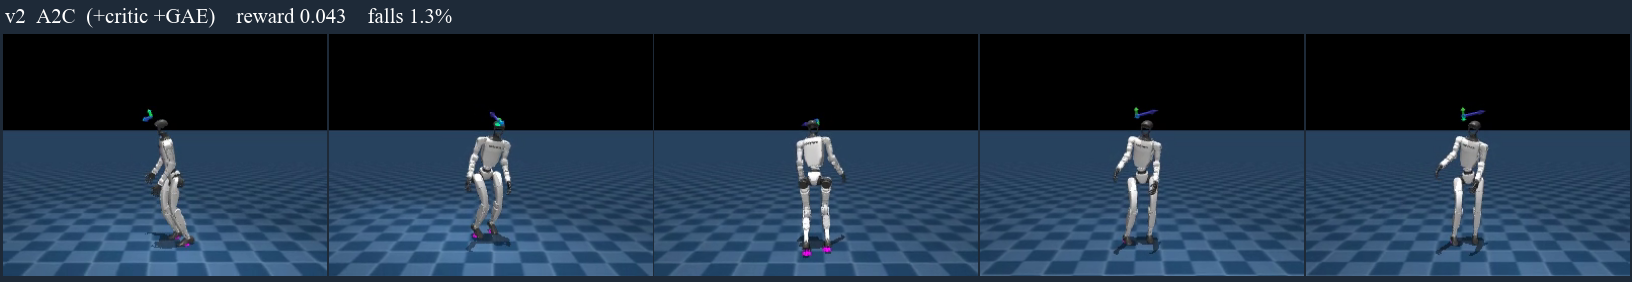
\includegraphics[width=0.98\linewidth,height=\textheight,keepaspectratio]{../../assets/figures/lecture14/ref/fig155-walk-v2.png}

}

\caption{v2 A2C 训练 3000 迭代后的 rollout
关键帧，从左到右为同一段时间内的连续时刻：G1 动作幅度比 v1
明显打开、姿态更舒展，但稳定性没有同步提高，偶有摔倒}

\end{figure}%

结果出乎意料：\textbf{评测奖励反而比 v1 低了}（0.043 对
0.070），摔倒率也没降。这不是
bug，是这一讲最好的教材，值得停下来仔细读：

\begin{itemize}
\tightlist
\item
  先说清一件容易夸大的事：方差被压低是 critic
  基线的\textbf{理论性质}（5.1
  节那个''减掉贴合状态的基线、不改变梯度期望却降方差''的结论），\textbf{不是}这张
  rollout
  对照图或''评测平均奖励''能直接证明的------真要验证方差降没降，得去看训练时的优势/梯度方差曲线。这张图能直接读到的是另一回事：v2
  的动作幅度比 v1
  大得多、姿态更舒展------评测记录里的动作绝对值均值也对得上，v2 是
  0.56，v1 与 v3 都是
  0.39。要当心的是，``动作更大''也不等于''探索更充分''：6.5
  节的策略熵曲线上 v2 反而比 v1 低（15 对
  22），也就是分布更窄、只是均值推得更远。梯度方差、动作幅度、分布宽度是三件事，别拿其中一件当另一件的证据。
\item
  但训练过程露出了一个 v1
  没有的故障模式：\textbf{单次更新会把刚学会的步态一脚踩塌}。看 6.5
  节那张训练奖励曲线：v2 的滑动平均在 0.004
  上下的平台上晃了两千多次迭代，而\textbf{第 500 迭代之后的这 2500
  次迭代}里，有 \textbf{195 次}迭代的平均奖励掉到 −0.01
  以下、最低一次掉到 −0.049；同一区间里 v1 最低只到 −0.0040，v3
  更是最低都还有 0.0189。
\end{itemize}

按理更干净的学习信号应当帮上忙，为什么反而更颠？\textbf{一个可能的解释}是：信号方差降低后，每次更新的推力更一致、有效步长变大------而这套算法里没有任何东西在管''一步最多能迈多大''。这只是一个解释，不是定论。要真正确认''栽跟头是因为步子太大''，需要的证据是：优势/梯度方差曲线、新旧策略的
KL、更新范数、学习率扫描，以及多个随机种子的对照------这些量在单次课堂预算的运行里看不到。支持这个解释的间接证据来自
v3：补上步长约束后，同样的优势估计立刻兑现成最高分，方向与''卡在步长''一致。

\subsection{5.6
毛病在哪：更新步子没人管}\label{ux6bdbux75c5ux5728ux54eaux66f4ux65b0ux6b65ux5b50ux6ca1ux4ebaux7ba1}

策略梯度只给方向，不给安全步长。学习率是固定的，优势偶尔被高估时，一次更新就可能把策略推得离原来很远------高斯分布的均值猛移、标准差猛缩，策略性格突变。

对 on-policy 方法（3.4
节）这尤其致命，因为它有个\textbf{恶性循环放大器}：策略被推坏了 →
下一轮只能用\textbf{被推坏的策略}采数据 → 数据也是坏的 →
在坏数据上更新，好不容易学到的东西被反复抹掉。v1
反而因为信号噪声大、单步推力互相抵消，误打误撞地''步子小''；v2
把噪声压干净，等于给车换了好引擎却没装刹车。

所以下一块要补的机制已经呼之欲出：\textbf{限制每次更新的步长}------这正是
PPO 的全部内容。

\subsection{5.7 本节小结}\label{ux672cux8282ux5c0fux7ed3-3}

A2C 在 REINFORCE 上补的是''参照物''：基线思想（跟平均比、不跟零比）→
理想基线就是状态价值 \(V^\pi(s)\) → 用 critic 网络去估它。与 REINFORCE
的分界线（本讲取窄定义）是 bootstrap：\(V\) 只当基线仍是 REINFORCE with
baseline，\(V\) 参与时序差分/GAE 估优势才是
actor-critic。两者用的是\textbf{同一条策略梯度公式}，只是权重从实际回报换成了评分员参与估计的优势。理论上
critic 基线会压低梯度方差（实验里能直接看到的只是动作幅度变大------0.56
对
0.39，这不等同于方差的证据）；本次运行中它没有步长约束，训练里有近两百次迭代被一次更新推坏，评测反而不如
v1（0.043 对 0.070）------这指向下一块拼图：管住步子。

\section{6
PPO：给更新步子加护栏}\label{ppoux7ed9ux66f4ux65b0ux6b65ux5b50ux52a0ux62a4ux680f}

\subsection{6.1 信赖域思想：TRPO 一句话，PPO
是它的好实现}\label{ux4fe1ux8d56ux57dfux601dux60f3trpo-ux4e00ux53e5ux8bddppo-ux662fux5b83ux7684ux597dux5b9eux73b0}

``每次更新别离旧策略太远''这个思想，学名叫\textbf{信赖域（trust
region）}：只在旧策略周围一小圈范围里更新，才信得过、不会崩。先把这个思想做严格的是
\textbf{TRPO}（Trust Region Policy Optimization）：用 KL
散度硬约束新旧策略的距离，再用二阶优化求解------理论漂亮，实现笨重。

\textbf{PPO}（Proximal Policy
Optimization，近端策略优化）{[}2{]}是它广为流传的简化版：``Proximal（近端）''说的就是新策略要待在旧策略附近。它不解带约束的优化问题，只在目标函数上动一个聪明的手脚------裁剪------一阶方法就能跑，效果却不输。稳定、通用、好实现，这让
PPO
长期是机器人控制与大模型对齐里的默认选择------大模型那边后来的变化，第15讲会讲。

\subsection{6.2 概率比值与 clip
目标}\label{ux6982ux7387ux6bd4ux503cux4e0e-clip-ux76eeux6807}

要约束''离旧策略多远''，先得有个量来度量它。PPO
用\textbf{新旧策略对同一个动作的概率比值}（提醒一句：这个 \(r\) 和 2.3
节那个奖励 \(r\)
只是恰好共用一个字母------一个是比值、一个是分数，文献里都这么写，别看串了）：

\[
r_t(\theta)=\frac{\pi_\theta(a_t\mid s_t)}{\pi_{\theta_{\text{old}}}(a_t\mid s_t)}
\]

\(r_t=1\) 表示新旧策略对这个动作看法一致；\(>1\)
是新策略更喜欢它，\(<1\) 是更嫌弃它。优势为正时我们想把 \(r_t\)
往上推，为负时往下压------但 PPO
不允许推拉得太夸张。它在目标函数里给这个比值套上一道
\([1-\epsilon,\,1+\epsilon]\) 的\textbf{裁剪（clip）}（\(\epsilon\) 取
0.2）：

\[
L^{\text{CLIP}}=\mathbb{E}\big[\min\big(r_t A_t,\ \text{clip}(r_t,1-\epsilon,1+\epsilon)\,A_t\big)\big]
\]

\begin{figure}[H]

{\centering 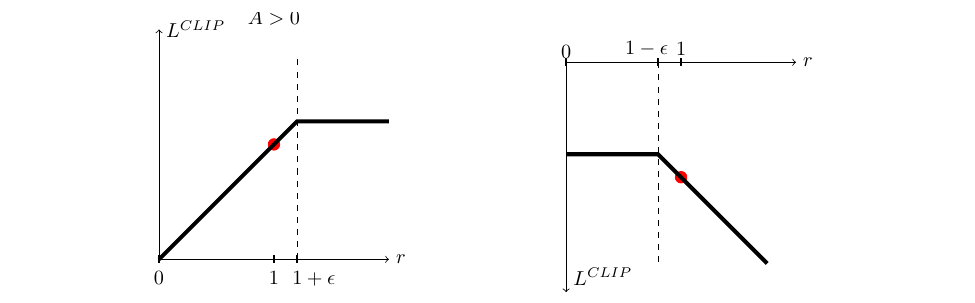
\includegraphics[width=0.8\linewidth,height=\textheight,keepaspectratio]{../../assets/figures/lecture14/ref/fig143-ppo-clip_arxiv-1707.06347.png}

}

\caption{PPO 的裁剪目标 \(L^{\text{CLIP}}\) 随概率比值 \(r\)
的变化：左图优势为正（好动作），右图优势为负（坏动作），红点是 \(r=1\)
的起点。\(r\)
一旦越过裁剪边界，目标就变平、梯度归零，更新自动失去动力。图出自参考文献
2 的图 1}

\end{figure}%

这张图分两种情况读：

\begin{itemize}
\tightlist
\item
  \textbf{左图（\(A>0\)，好动作）}：想增大概率、把 \(r\) 往右推；但
  \(r\) 一旦越过
  \(1+\epsilon\)，曲线就\textbf{变平}------再推目标也不涨，梯度归零，更新自动停手，好动作的概率不会被推到离谱。
\item
  \textbf{右图（\(A<0\)，坏动作）}：对称地想把 \(r\) 往左压；越过
  \(1-\epsilon\) 后曲线同样变平，不会一脚把坏动作踩到零。
\end{itemize}

以 \(\epsilon=0.2\) 说人话：一旦新策略把某个动作的概率推出旧策略的 0.8
到 1.2 倍，目标函数就不再奖励继续推。要点在于------\textbf{clip
夹的是''目标函数的收益''，不是硬卡住比值 \(r_t\) 本身}：某个样本的
\(r_t\)
仍然可能越过这个区间，只是越界之后再推也赚不到分、梯度归零。\textbf{``走太远''在目标函数里赚不到钱，每次更新于是很少跑得太离谱。}

\begin{quote}
备注：所以 PPO-Clip
只是一道\textbf{软}信赖域------它是在代理目标上做的软约束，\textbf{不保证}策略始终待在一个严格的信赖域里。它不像
TRPO 那样用 KL
硬约束新旧策略的距离，只是让越界的更新''无利可图''；实际训练中 KL
仍可能超标，\(r_t\) 也可能被别的样本带出区间。正因为 clip
不是铁栅栏，工业级 PPO 才要再配 6.3 节的 KL 自适应学习率兜底，并持续监控
KL、策略熵和梯度范数。本讲后文说''夹进信赖域''，都是这个软的意思。
\end{quote}

\subsection{6.3 数据复用与 KL
自适应}\label{ux6570ux636eux590dux7528ux4e0e-kl-ux81eaux9002ux5e94}

clip 还带来一个重要副产品：\textbf{同一批数据可以多用几遍了}。没有 clip
时数据基本只敢用一遍------多用几遍策略就被推飞；有 clip
抑制过大的概率比更新，PPO 就能把一段 rollout
拆成几份\textbf{小批（minibatch）}、再把整段数据反复过上好几个
epoch，样本效率大幅提高，顺手缓解了 on-policy
费样本的老毛病。（这是''通常更稳''，不是安全保证------KL
仍可能超标，所以要监控，下面就说这件事。）

工业级 PPO 通常还加一个自动化步长管家：\textbf{按 KL
散度自适应学习率}------每次更新后量一下新旧策略的 KL 距离，动得太猛（KL
超标）就调小学习率，动得太小就调大，步长自动收放。至此，一轮完整的 PPO
训练是：

\begin{enumerate}
\def\labelenumi{\arabic{enumi}.}
\tightlist
\item
  用当前策略采一批 rollout；
\item
  critic + GAE 算每步优势 \(A_t\)（第 5 节原样保留）；
\item
  切成多个 minibatch，用 \(L^{\text{CLIP}}\) 反复更新多轮，同时用 value
  loss 更新 critic；
\item
  按 KL 调学习率，回到第 1 步。
\end{enumerate}

\subsection{6.4 代码走读：v2 到 v3
改了什么}\label{ux4ee3ux7801ux8d70ux8bfbv2-ux5230-v3-ux6539ux4e86ux4ec0ux4e48}

\texttt{code/rl/1\_rl\_basics/1\_1\_g1\_walk\_rl/train\_v3\_ppo.py} 在
v2 上加三块，正好对应上两节。第一块，policy loss
换成裁剪目标------采样时顺手记下旧策略的
\texttt{log\_probs}，训练时算比值：

\begin{Shaded}
\begin{Highlighting}[]
\CommentTok{\# 关键变化(1)：clip——用概率比值把更新夹在信赖域内（见 6.2 节的图）}
\NormalTok{        ratio }\OperatorTok{=}\NormalTok{ torch.exp(log\_probs }\OperatorTok{{-}}\NormalTok{ batch[}\StringTok{"log\_probs"}\NormalTok{])}
\NormalTok{        unclipped }\OperatorTok{=}\NormalTok{ ratio }\OperatorTok{*}\NormalTok{ batch[}\StringTok{"advantages"}\NormalTok{]}
\NormalTok{        clipped }\OperatorTok{=}\NormalTok{ (torch.clamp(ratio, }\FloatTok{1.0} \OperatorTok{{-}} \VariableTok{self}\NormalTok{.clip\_param, }\FloatTok{1.0} \OperatorTok{+} \VariableTok{self}\NormalTok{.clip\_param)}
                   \OperatorTok{*}\NormalTok{ batch[}\StringTok{"advantages"}\NormalTok{])}
\NormalTok{        policy\_loss }\OperatorTok{=} \OperatorTok{{-}}\NormalTok{torch.}\BuiltInTok{min}\NormalTok{(unclipped, clipped).mean()}
\end{Highlighting}
\end{Shaded}

第二块在数据端：\texttt{G1WalkRolloutDataset} 不再把整段 rollout
打包成一个 batch 用一遍，而是切成 minibatch、重复多个 epoch
逐个吐出------Lightning 那边一行不用改，多轮复用完全由数据集实现：

\begin{Shaded}
\begin{Highlighting}[]
\CommentTok{\# 关键变化(2)：一段 rollout 切成多个 minibatch、反复训几轮，样本效率更高}
        \ControlFlowTok{for}\NormalTok{ \_ }\KeywordTok{in} \BuiltInTok{range}\NormalTok{(}\VariableTok{self}\NormalTok{.num\_learning\_epochs):}
\NormalTok{            indices }\OperatorTok{=}\NormalTok{ torch.randperm(usable\_size, device}\OperatorTok{=}\NormalTok{flat[}\StringTok{"actions"}\NormalTok{].device)}
            \ControlFlowTok{for}\NormalTok{ start }\KeywordTok{in} \BuiltInTok{range}\NormalTok{(}\DecValTok{0}\NormalTok{, usable\_size, mini\_batch\_size):}
\NormalTok{                selected }\OperatorTok{=}\NormalTok{ indices[start : start }\OperatorTok{+}\NormalTok{ mini\_batch\_size]}
\NormalTok{                mini\_batch }\OperatorTok{=}\NormalTok{ \{key: value[selected] }\ControlFlowTok{for}\NormalTok{ key, value }\KeywordTok{in}\NormalTok{ flat.items()\}}
\end{Highlighting}
\end{Shaded}

第三块是步长管家，挂在 Lightning 的 \texttt{on\_before\_optimizer\_step}
钩子上：

\begin{Shaded}
\begin{Highlighting}[]
\CommentTok{\# 关键变化(3)：按 KL 自适应调学习率——动得太猛减速，太小加速}
\KeywordTok{def}\NormalTok{ adapt\_learning\_rate\_to\_kl(optimizer, kl, desired\_kl, min\_lr}\OperatorTok{=}\FloatTok{1.0e{-}5}\NormalTok{, max\_lr}\OperatorTok{=}\FloatTok{1.0e{-}2}\NormalTok{):}
\NormalTok{    current\_lr }\OperatorTok{=}\NormalTok{ optimizer.param\_groups[}\DecValTok{0}\NormalTok{][}\StringTok{"lr"}\NormalTok{]}
\NormalTok{    kl\_value }\OperatorTok{=} \BuiltInTok{float}\NormalTok{(kl.detach().cpu())}
    \ControlFlowTok{if}\NormalTok{ kl\_value }\OperatorTok{\textgreater{}} \FloatTok{2.0} \OperatorTok{*}\NormalTok{ desired\_kl:}
\NormalTok{        current\_lr }\OperatorTok{=} \BuiltInTok{max}\NormalTok{(min\_lr, current\_lr }\OperatorTok{/} \FloatTok{1.5}\NormalTok{)}
    \ControlFlowTok{elif} \FloatTok{0.0} \OperatorTok{\textless{}}\NormalTok{ kl\_value }\OperatorTok{\textless{}} \FloatTok{0.5} \OperatorTok{*}\NormalTok{ desired\_kl:}
\NormalTok{        current\_lr }\OperatorTok{=} \BuiltInTok{min}\NormalTok{(max\_lr, current\_lr }\OperatorTok{*} \FloatTok{1.5}\NormalTok{)}
\NormalTok{    optimizer.param\_groups[}\DecValTok{0}\NormalTok{][}\StringTok{"lr"}\NormalTok{] }\OperatorTok{=}\NormalTok{ current\_lr}
    \ControlFlowTok{return}\NormalTok{ current\_lr}
\end{Highlighting}
\end{Shaded}

此外 v3 对 value loss 也做了对称的裁剪（新估值别离旧估值太远），思路与
clip 一脉相承。这套''clip + 多轮复用 + KL
自适应''不是本课程自创的组合：它逐条对得上 mjlab 给宇树 G1
速度跟随任务备好的官方 PPO 配方{[}7{]}，而 BeyondMimic{[}4{]} 训练真机
G1
的动作跟踪策略走的也是同一条路子------等下我们原样把它搬去做更难的任务。

\subsection{6.5
实验：三个算法同台，行走任务收口}\label{ux5b9eux9a8cux4e09ux4e2aux7b97ux6cd5ux540cux53f0ux884cux8d70ux4efbux52a1ux6536ux53e3}

三个版本到齐，统一口径最后对照一次：

\begin{center}
\begin{tabular}{@{}>{\raggedright\arraybackslash}p{\dimexpr 0.0938\linewidth - 2\tabcolsep\relax} >{\raggedright\arraybackslash}p{\dimexpr 0.4844\linewidth - 2\tabcolsep\relax} >{\raggedright\arraybackslash}p{\dimexpr 0.2188\linewidth - 2\tabcolsep\relax} >{\raggedright\arraybackslash}p{\dimexpr 0.1250\linewidth - 2\tabcolsep\relax}@{}}
\toprule\noalign{}
版本 & 算法 & 评测平均奖励 & 摔倒率 \\
\midrule\noalign{}
v1 & REINFORCE & 0.070 & 1.3\% \\
v2 & A2C（+critic +GAE） & 0.043 & 1.3\% \\
\textbf{v3} & \textbf{PPO（+clip +复用 +KL 自适应）} & \textbf{0.097} & \textbf{0.0\%} \\
\bottomrule\noalign{}
\end{tabular}
\end{center}

\begin{figure}[H]

{\centering 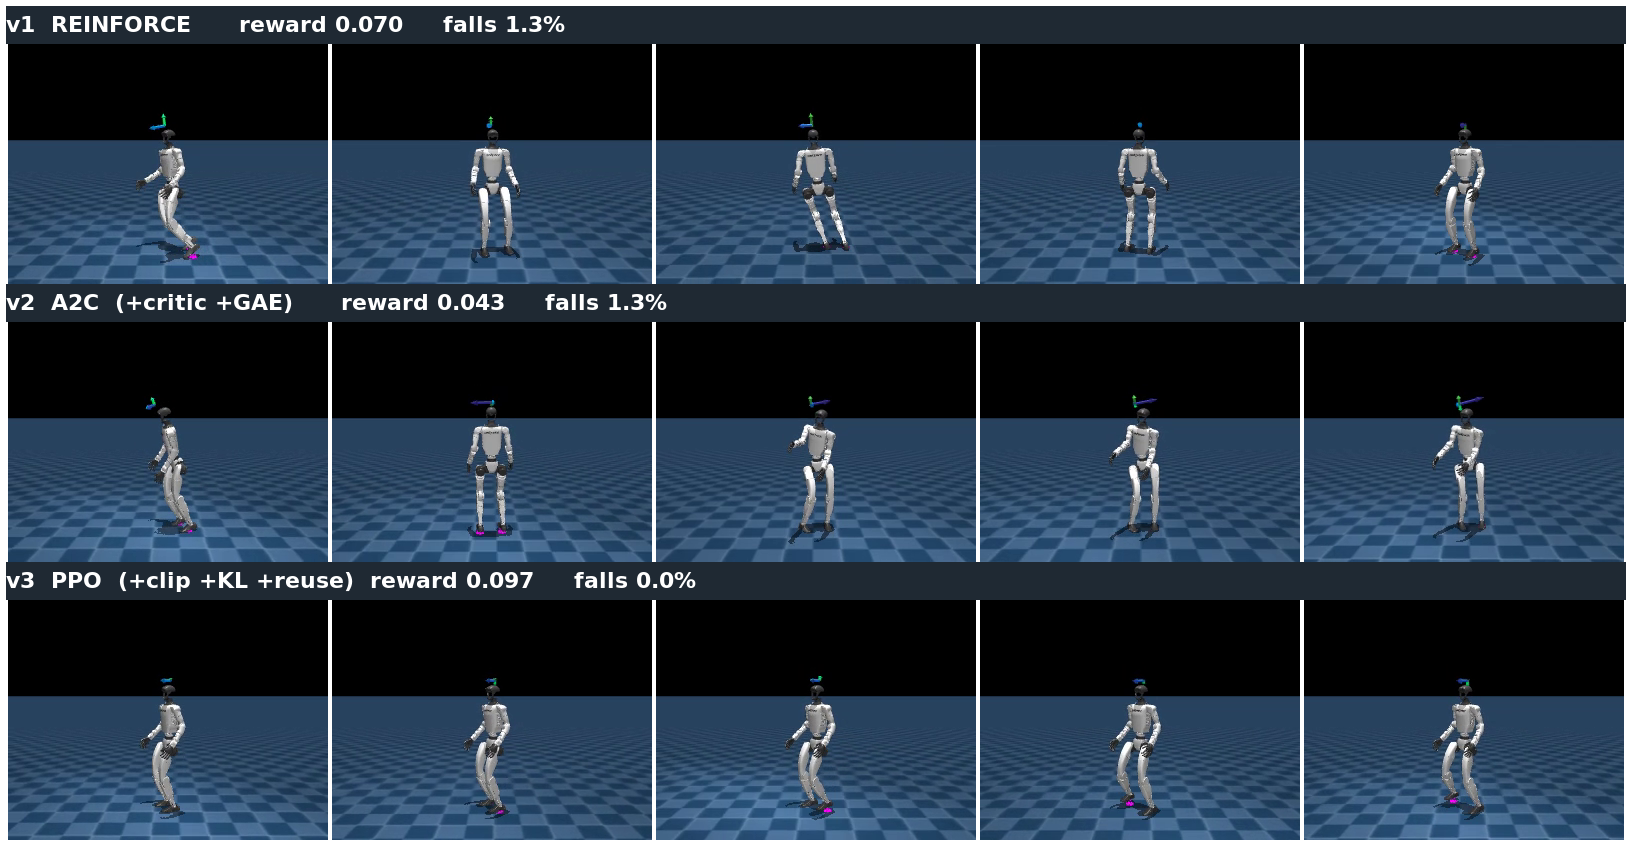
\includegraphics[width=0.98\linewidth,height=\textheight,keepaspectratio]{../../assets/figures/lecture14/ref/fig144-walk-compare.png}

}

\caption{G1 行走三算法 rollout
对照，每行从左到右是同一段时间内的关键帧，从上到下依次为 v1
REINFORCE、v2 A2C、v3 PPO；各行标题上印着该版本的评测奖励与摔倒率。v3
全程直立稳定，6400 个评测步里一次都没倒}

\end{figure}%

表格和截图给的是终点成绩，把整个训练过程画出来，三者的差别更直白：

\begin{figure}[H]

{\centering 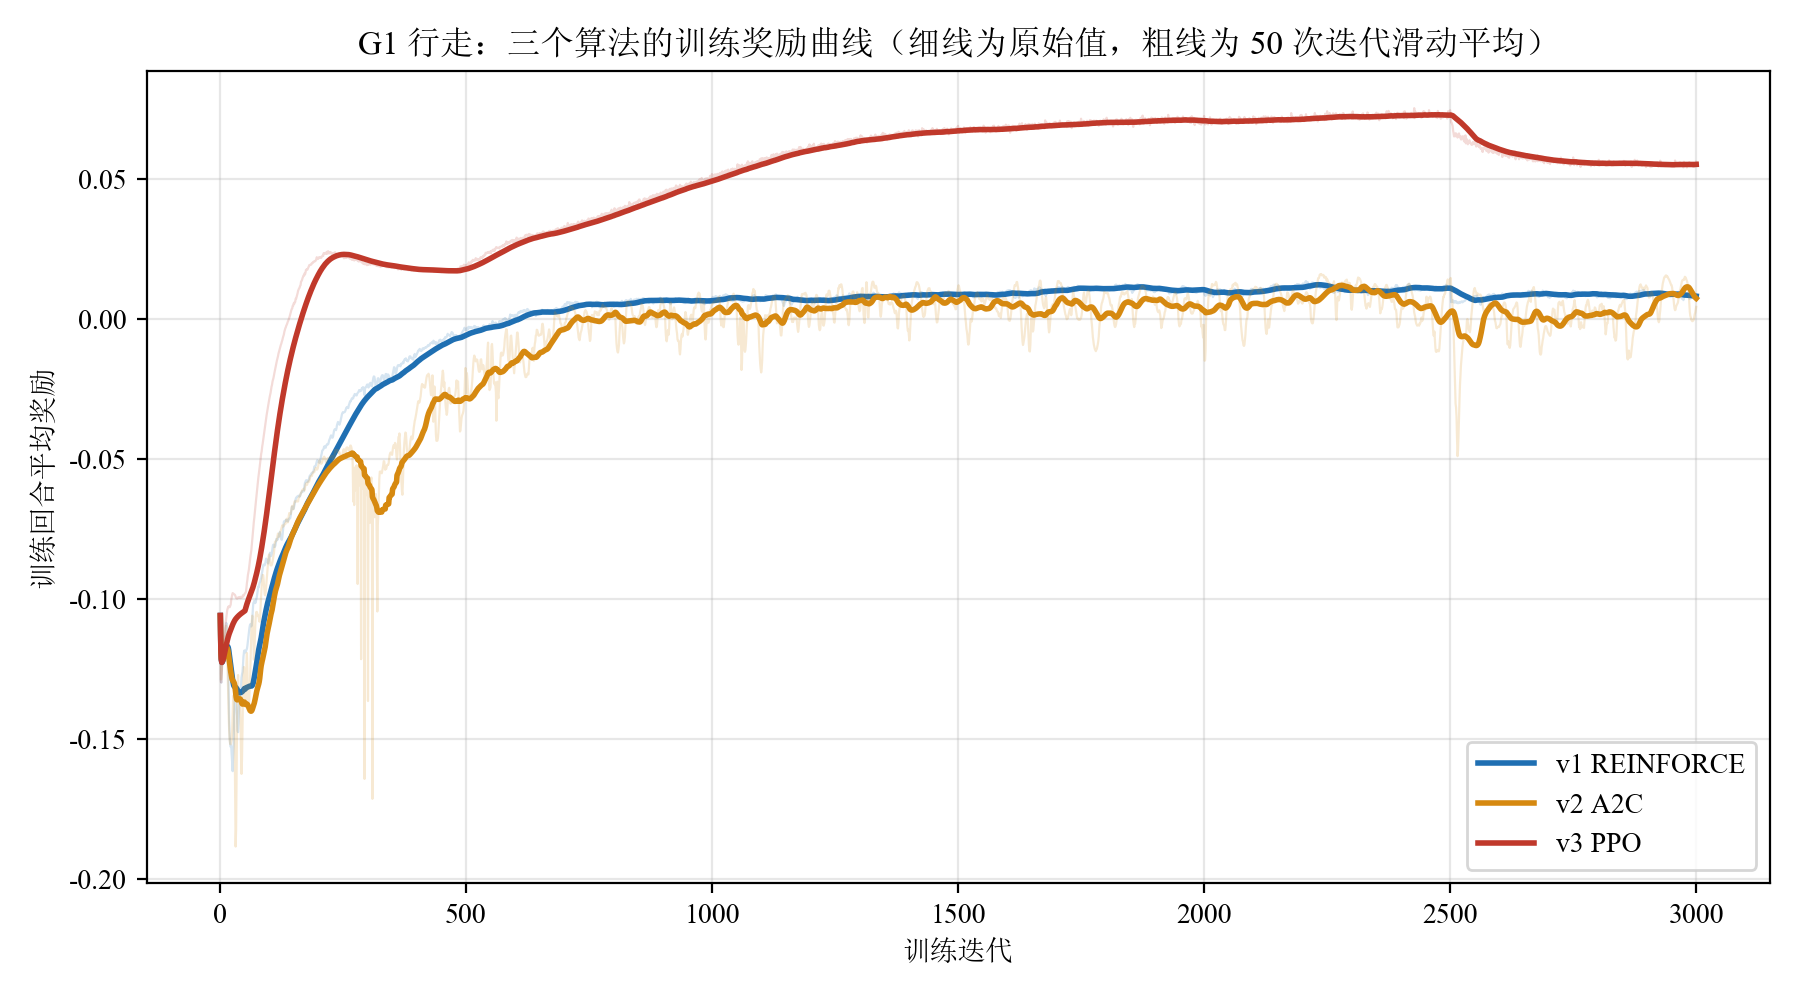
\includegraphics[width=0.96\linewidth,height=\textheight,keepaspectratio]{../../assets/figures/lecture14/ref/fig146-train-reward-curves.png}

}

\caption{G1 行走三算法的训练奖励曲线（同为 3000
次迭代，细线为每次迭代的原始值，粗线为 50 次迭代的滑动平均）：v3 PPO
爬到 0.073 附近，在约 2500 迭代处掉了一级、余下区间稳在 0.055；v1 与 v2
大约 700 迭代后就压在 0 附近再没上去，v2
的原始曲线抖动幅度最大。数据来源：\texttt{code/rl/1\_rl\_basics/result/1\_1\_g1\_walk\_rl/train-reward-curves.json}}

\end{figure}%

这张图要分两层读。\textbf{细线是每次迭代的原始奖励，粗线是它的趋势}。先看细线：真正一直毛刺丛生的只有
v2，后 2500 次迭代里它的原始值与滑动平均平均差 0.0046，而 v1 和 v3
的细线都紧贴着各自的粗线（0.0007 与
0.0009）。这里要防一个很容易犯的误读：\textbf{REINFORCE
的高方差大在梯度上，不在这条曲线上}------曲线画的是 4096
个环境的平均奖励，几万条样本一平均，逐次迭代之间本来就不会抖；4.7
节那个方差说的是同一批数据里每个动作拿到的权重有多散，这张图证不了它（5.5
节已经提醒过同样的陷阱，只是方向相反）。v2
的细线之所以抖，是它每一步真的把策略推得忽左忽右。

\textbf{趋势那一层才是三者的差距所在}：v1 和 v2 大约 700
次迭代后就双双卡在 0 附近再也上不去（末段滑动平均 0.008 与 0.007），v2
还更低一点；v3 一路爬到 0.073，把另外两条甩开近一个量级------这正是 5.6
节说的''更新步子没人管''与''管住了''的区别。

不过 v3 这条线在 2500 迭代前后\textbf{掉了一级}：滑动平均从 0.073 落到
0.055，之后再没回去。这不违背 6.2 节那条备注------clip
是软约束不是铁栅栏，单次运行里出现这种回落并不稀奇。本讲不替它编一个原因：要定性得靠多个随机种子和更细的诊断量，超出课堂预算。记住这个时间点，读下一张损失图时它还会再出现一次。

训练时记下的各项损失，则从另一个角度说明了三版到底各自在优化什么：

\begin{figure}[H]

{\centering 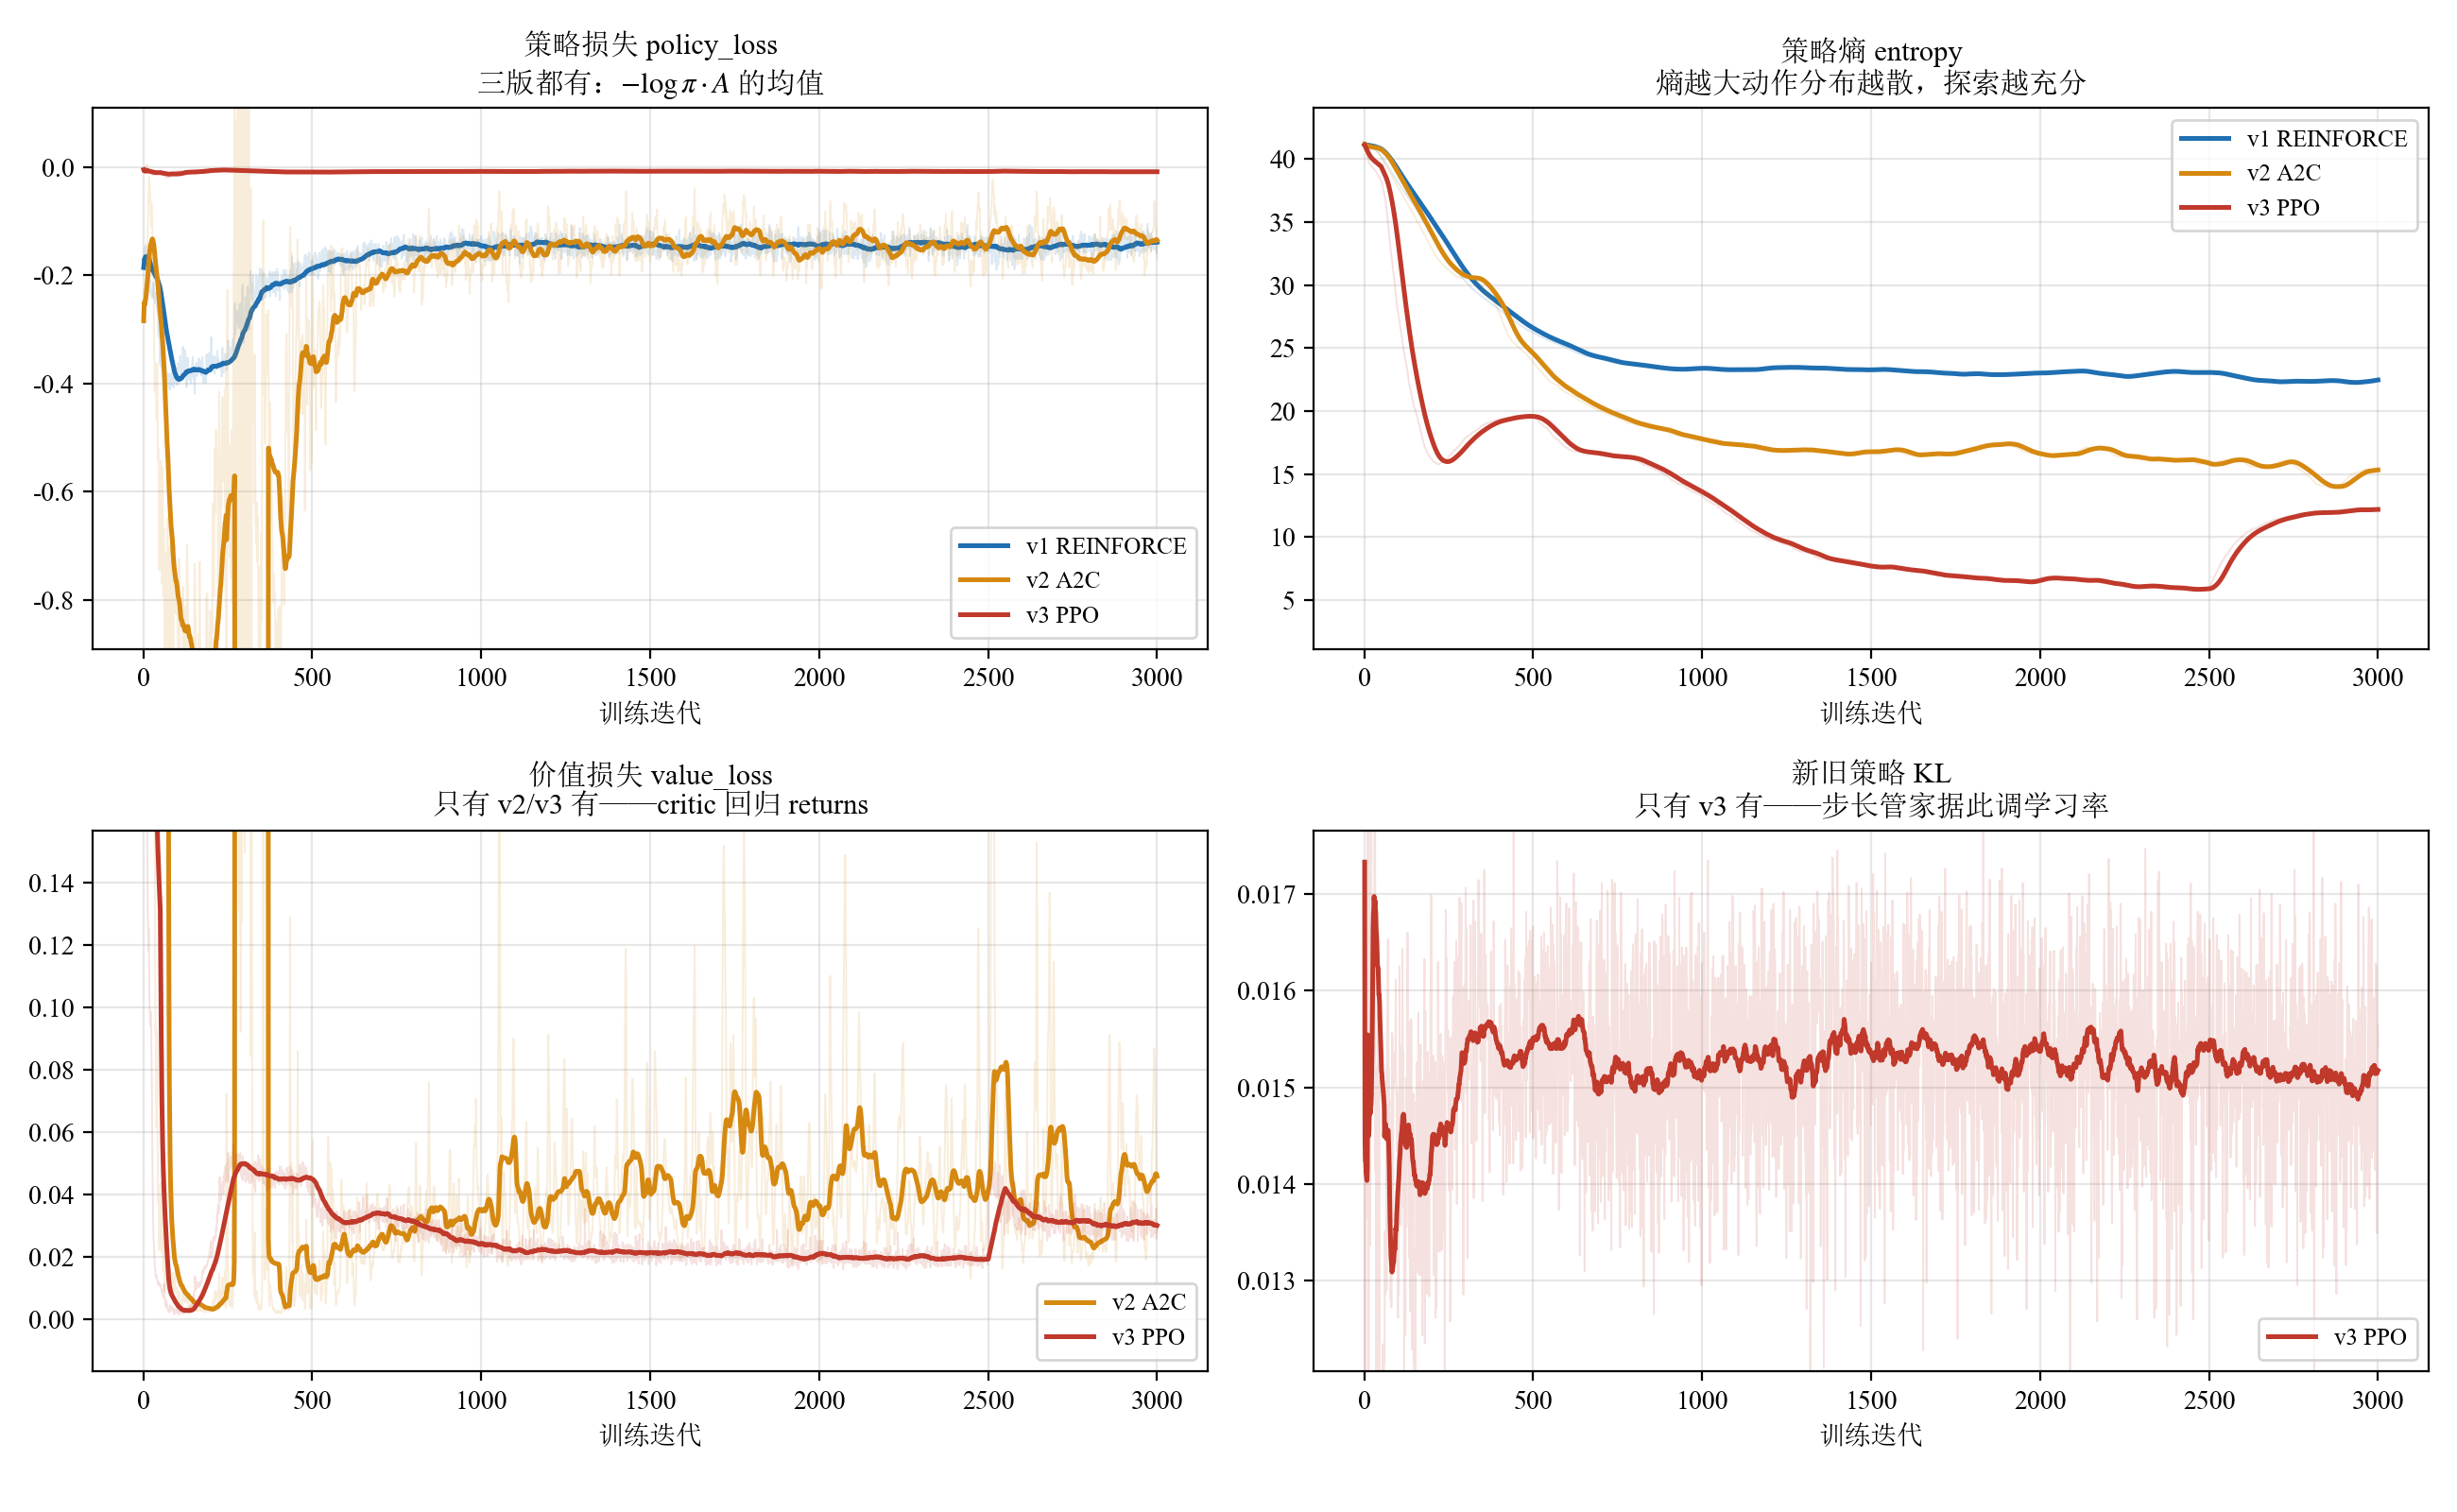
\includegraphics[width=0.98\linewidth,height=\textheight,keepaspectratio]{../../assets/figures/lecture14/ref/fig146-train-loss-curves.png}

}

\caption{G1 行走三算法的训练损失（细线为每次迭代原始值，粗线为 50
次迭代滑动平均）：左上策略损失三版都有；右上策略熵反映探索强度；左下价值损失只有
v2/v3 有；右下新旧策略 KL 只有 v3
记录。数据来源：\texttt{code/rl/1\_rl\_basics/result/1\_1\_g1\_walk\_rl/train-loss-curves.json}}

\end{figure}%

四个面板正好对应三版的差异。\textbf{策略损失}三版都有，但只看它没用------它的绝对值不能横向比较，因为每版的优势估计口径不同。\textbf{策略熵}最能说明问题：三条线都从
41 附近往下走（策略逐渐变确定），但走的节奏差很多------v1
降得最慢、末段仍停在 22 以上，说明它的动作分布一直很散、迟迟收不拢；v2
收到 15 附近；v3 一路压到
5.9（三者中最低），动作最果断。（熵说的是分布\textbf{摊得多宽}，和 5.5
节那个''动作幅度''不是一回事------后者量的是均值有多大，所以熵最高的 v1
反而动作最小。）注意 v3 的熵在 2500 迭代之后\textbf{又反弹回 12
附近}，和上一张图那次回落是同一个时间点------同一件事在两张图上都留下了痕迹。

下面两个面板只有部分版本有。\textbf{价值损失}只有 v2 和 v3 有，因为 v1
根本没训 critic：v3 的一路降到 0.02 上下，但在 2500
迭代前后同样跳了一级、末段停在 0.030------又是那个时间点；v2 的则从 700
迭代时的 0.027 起起落落地涨到末段的
0.046。价值损失升高不等于评分员变笨------它要拟合的目标（回报）本身也随策略在变------但至少可以确定一件事：这两条线\textbf{并不都是''稳定收敛''}，所以想拿它来断言''A2C
卡住与 critic 无关''，证据是不够的，5.5
节那个解释仍然只是解释。\textbf{新旧策略 KL} 只有 v3 记录，全程稳定在
0.015 附近（目标值 0.01）------图上那条 50
次迭代滑动平均的粗线整段都落在 0.013 到 0.018
之间，抖得最厉害的单次迭代也不过 0.028。这正是步长管家在起作用：KL
偏大就压学习率、偏小就放开。

v3 把两个指标同时拿下：评测奖励最高（0.097），\textbf{摔倒率归零}。它对
5.5 节那个反常结果给出的回收是：同一套 critic + GAE
的优势估计，配上步长约束之后立刻兑现成了最高分------这支持''卡脖子的主要是步长''这个方向。但按上面价值损失那条线看，也不能反过来说
v2 的 critic 一点问题没有。

值得留意的是，v3 其实比 v2 训得\textbf{更激进}：同一批数据训 5 个
epoch、每个 epoch 切 4 份 minibatch，一共 20 个优化
step（\textbf{单个样本约被用 5 次}，不是 20 次------每个 epoch
里每个样本只出现在一份 minibatch 里），而 v2
只过一遍。更激进却更稳，是因为 clip
把每次更新的概率比压在了一个小区间里。\textbf{护栏不是让车变慢，是让车敢开快。}

\begin{quote}
备注：3000
迭代的课堂预算下，三者都还停留在''稳住、小幅行走''而非利落快走------mjlab
官方那份 G1 配方把迭代次数设在 \textbf{3
万}{[}7{]}，是这里的十倍。本实验的目的是对照算法差异，不是刷行走质量；把
\texttt{max\_iterations} 调大即可提升绝对效果，算法本身不用动。
\end{quote}

\subsection{6.6
实验加码：把同一套算法搬去做动作跟随}\label{ux5b9eux9a8cux52a0ux7801ux628aux540cux4e00ux5957ux7b97ux6cd5ux642cux53bbux505aux52a8ux4f5cux8ddfux968f}

行走任务上三版好歹都能站住，光看 rollout
截图差距还不算触目。把同一套代码搬到一个\textbf{难得多}的任务上试试：让
G1 \textbf{逐帧贴住一段真实武术动作}------参考动作由真人视频重定向到 G1
得到，用的正是 4.4 节认识的那条管线：GVHMR 从视频恢复人体动作，GMR
把它重定向成 G1
的参考轨迹。它比走路难在目标上：不再是''别摔就行''，而是每一帧都要匹配参考姿态。这一组的代码在
\texttt{code/rl/1\_rl\_basics/1\_3\_g1\_motion\_tracking/}，三个版本与行走线一一对应，只把环境从速度指令换成了参考动作跟踪；评测摘要同样落在
\texttt{code/rl/1\_rl\_basics/result/1\_3\_g1\_motion\_tracking/} 下的
\texttt{.json} 里。

这正是 BeyondMimic{[}4{]} 做的事情------同一套 PPO 配方，训练真实宇树 G1
做出空中侧手翻、旋踢、翻身踢、冲刺这类敏捷动作：

\begin{figure}[H]

{\centering 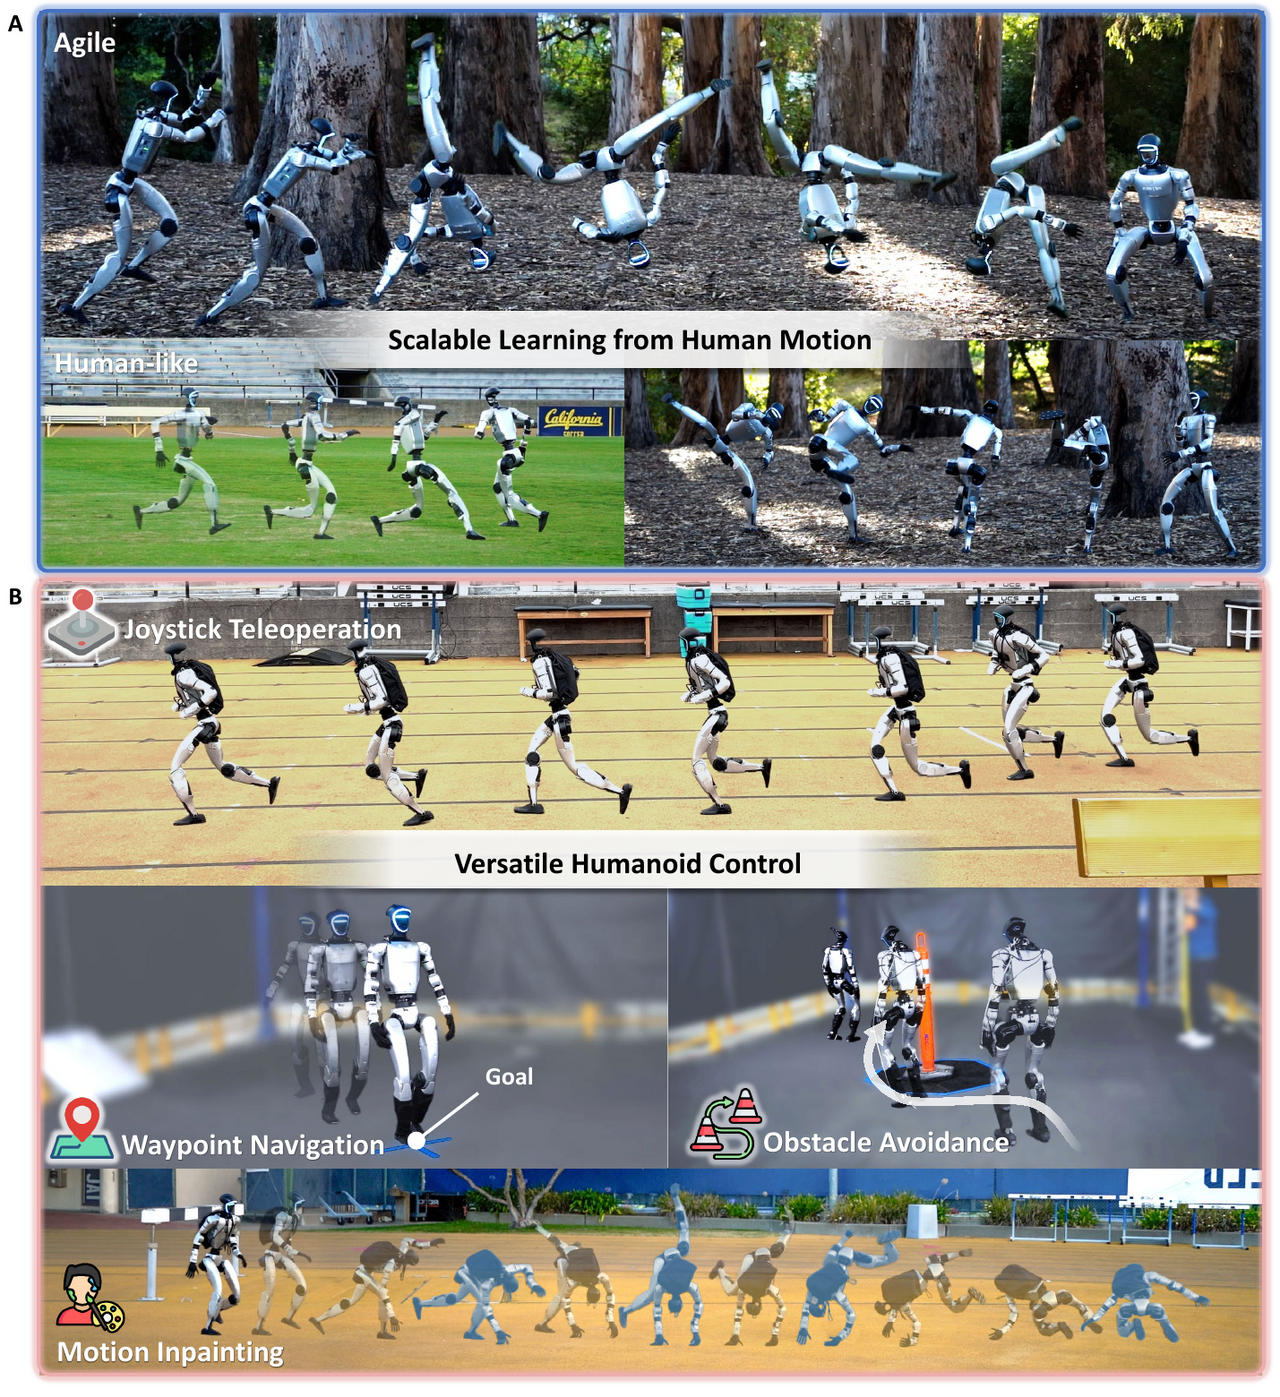
\includegraphics[width=0.7\linewidth,height=\textheight,keepaspectratio]{../../assets/figures/lecture14/ref/fig144-beyondmimic-real_arxiv-2508.08241.png}

}

\caption{BeyondMimic 在真实宇树 G1
上的效果：上半格（A）是从人体动作中学到的敏捷与拟人动作，本讲搬用的就是这一半；下半格（B）是它在动作跟踪之上再套一层扩散模型之后才支持的手柄遥操、路点导航、避障与动作补全，不在本讲范围。图出自参考文献
4}

\end{figure}%

\begin{quote}
备注：本讲借用的是 BeyondMimic
的\textbf{动作跟随}那一半------让机器人稳稳执行给定的动捕轨迹，而不是凭空''涌现''出跑酷。这一点要说清楚，免得对强化学习的能力产生误解：难点在控制，不在动作创意。
\end{quote}

仿真里跑同样的三档，但要先把口径讲清楚：\textbf{这一组不是公平的算法对照。}
v3 直接复用了原版 PPO 训到 10000 迭代的权重，而 v1/v2 只训了 3000
迭代------训练预算差了三倍多，算法差异和训练时长差异混在了一起。所以下表应当读作''\textbf{各版本最终可用
checkpoint 的展示}''，不能用来支撑''算法 A 强于算法 B''：

\begin{center}
\begin{tabular}{@{}>{\raggedright\arraybackslash}p{\dimexpr 0.0938\linewidth - 2\tabcolsep\relax} >{\raggedright\arraybackslash}p{\dimexpr 0.3750\linewidth - 2\tabcolsep\relax} >{\raggedright\arraybackslash}p{\dimexpr 0.2188\linewidth - 2\tabcolsep\relax} >{\raggedright\arraybackslash}p{\dimexpr 0.1250\linewidth - 2\tabcolsep\relax}@{}}
\toprule\noalign{}
版本 & 算法（训练预算） & 评测平均奖励 & 摔倒率 \\
\midrule\noalign{}
v1 & REINFORCE（3000 迭代） & 0.052 & 2.6\% \\
v2 & A2C（3000 迭代） & 0.046 & 1.2\% \\
\textbf{v3} & \textbf{PPO 原版（10000 迭代）} & \textbf{0.070} & \textbf{0.0\%} \\
\bottomrule\noalign{}
\end{tabular}
\end{center}

\begin{figure}[H]

{\centering 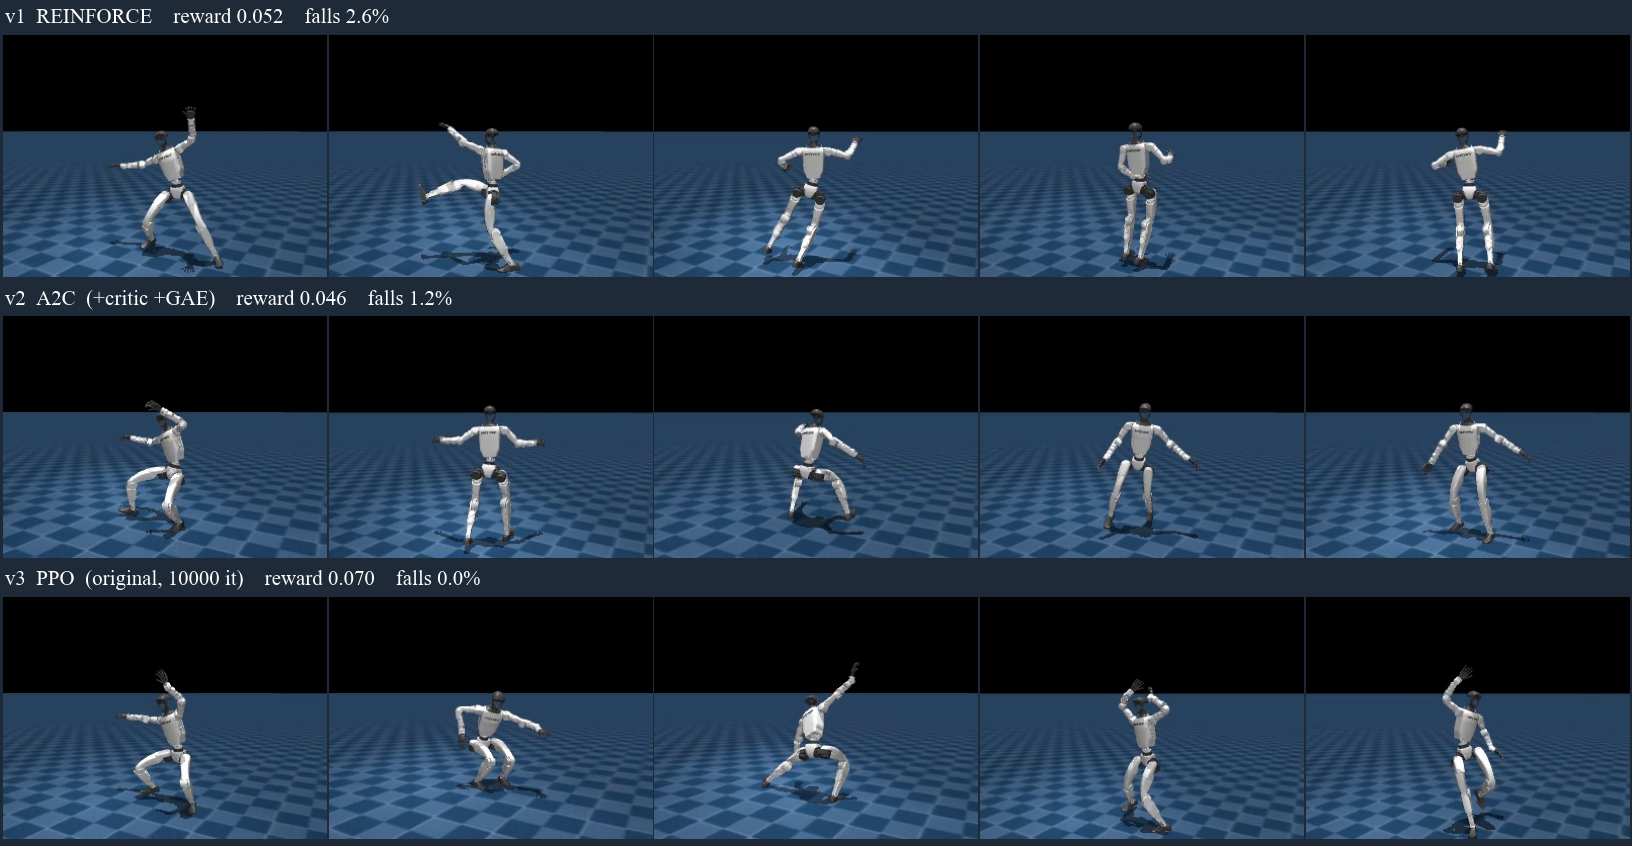
\includegraphics[width=0.98\linewidth,height=\textheight,keepaspectratio]{../../assets/figures/lecture14/ref/fig144-track-compare.png}

}

\caption{G1 动作跟随三算法 rollout
对照，每行从左到右是同一段时间内的关键帧，从上到下依次为 v1
REINFORCE、v2 A2C、v3 PPO；各行标题上写着该版本的评测奖励与摔倒率（v3 的
0.0\% 是四舍五入，6400 个评测步里实际倒了 1
次）。\textbf{画面里只有机器人自己，参考动作没有画进来}，数据来源是
\texttt{code/rl/1\_rl\_basics/result/1\_3\_g1\_motion\_tracking/}
下的三份评测记录。\textbf{画面里只有机器人自己，参考动作没有画进来}，所以这张图能直接看的是三者都还站得住、都在做幅度不小的武术式动作；跟得准不准要看奖励数字}

\end{figure}%

这张图给得出的只有一句：三个版本都没当场瘫倒。\textbf{跟得准不准它给不了}------参考姿态没有画进画面，差别只能从跟随奖励上读：0.070
对 0.052 /
0.046。受上面那条预算不对齐的限制，这三个数也只支持一句保守的观察：在各自这个预算下，完整
PPO
的最终权重在硬任务上拿到了明显更高的跟随奖励。想把它坐实成''任务越难、差距越大''，还得统一环境步数
/ 墙钟 / 优化 step
再跑多个随机种子。真正预算对齐的对照是行走任务那组（6.5 节，三者同为
3000 迭代）。

\begin{quote}
备注（本讲实验结论的效力边界）：6.5
节与本节的数字都来自\textbf{单次训练、单次评测}，没有多随机种子、没有置信区间，评测回合数也有限；rollout
截图只是定性展示，不能替代统计。要把这类对照写进正式结论，标准做法是：报告训练曲线的均值
± 标准差（至少 3\textasciitilde5 个种子）、评测至少 100
回合并给出成功率区间、公开评测脚本与 checkpoint
的选取规则。本讲的目的是让你看清三个算法\textbf{机制上}的差别，教学演示的数字请按''本次运行观察到''来读。
\end{quote}

\subsection{6.7 本节小结}\label{ux672cux8282ux5c0fux7ed3-4}

PPO 在 A2C 之上补的是''步长安全''：用概率比值 \(r_t\) 度量策略变化，clip
让''走太远''无利可图，软性地把更新压在旧策略附近；有 clip
抑制过大更新才敢多轮复用数据，再加 KL
自适应学习率自动收放步长。在同预算的行走任务对照里（6.5 节），本次运行中
v3 同时拿下最高奖励与零摔倒，回收了 v2 的反常；动作跟随任务上 PPO
的最终权重拿到了明显更高的跟随奖励（注意那一组训练预算不对齐，见 6.6
节）。

\section{7 本讲小结}\label{ux672cux8bb2ux5c0fux7ed3}

\subsection{7.1
一条演进链：每一步为什么发生}\label{ux4e00ux6761ux6f14ux8fdbux94feux6bcfux4e00ux6b65ux4e3aux4ec0ux4e48ux53d1ux751f}

回看整条路，每个算法都是被前一个的毛病\textbf{逼}出来的：

\begin{center}
\begin{tabular}{@{}>{\raggedright\arraybackslash}p{\dimexpr 0.0757\linewidth - 2\tabcolsep\relax} >{\raggedright\arraybackslash}p{\dimexpr 0.1629\linewidth - 2\tabcolsep\relax} >{\raggedright\arraybackslash}p{\dimexpr 0.3765\linewidth - 2\tabcolsep\relax} >{\raggedright\arraybackslash}p{\dimexpr 0.2647\linewidth - 2\tabcolsep\relax} >{\raggedright\arraybackslash}p{\dimexpr 0.1202\linewidth - 2\tabcolsep\relax}@{}}
\toprule\noalign{}
版本 & 算法 & 新增机制 & 解决什么毛病 & 对应章节 \\
\midrule\noalign{}
v1 & REINFORCE & 策略梯度 + reward-to-go & ------（起点） & 第 4 节 \\
v2 & A2C & critic 基线 + GAE 优势 & v1 回报噪声大（方差） & 第 5 节 \\
v3 & PPO & clip + 多轮复用 + KL 自适应 & v2 更新步长没人管 & 第 6 节 \\
\bottomrule\noalign{}
\end{tabular}
\end{center}

一轮完整 PPO 的数据流也顺一遍：当前策略在 4096 个并行环境里采 24 步 →
critic + GAE 把每步的优势估出来 → 切成 4 份 minibatch 反复训 5
轮，policy loss 走 clip、value loss 回归回报 → 按 KL 调学习率 →
丢掉数据，用新策略再采。本讲的关键超参数一览：

\begin{center}
\begin{tabular}{@{}>{\raggedright\arraybackslash}p{\dimexpr 0.4375\linewidth - 2\tabcolsep\relax} >{\raggedright\arraybackslash}p{\dimexpr 0.2812\linewidth - 2\tabcolsep\relax} >{\raggedright\arraybackslash}p{\dimexpr 0.2188\linewidth - 2\tabcolsep\relax}@{}}
\toprule\noalign{}
超参数 & 取值 & 在哪一节出现 \\
\midrule\noalign{}
折扣因子 \(\gamma\) & 0.99 & 2.3 节 \\
GAE 系数 \(\lambda\) & 0.95 & 5.3 节 \\
clip 范围 \(\epsilon\) & 0.2 & 6.2 节 \\
复用轮数 × minibatch 数 & 5 × 4 & 6.3 节 \\
目标 KL（学习率自适应） & 0.01 & 6.3 节 \\
熵奖励系数 & 0.01 & 4.5 节 \\
并行环境 × 每轮步数 × 迭代 & 4096 × 24 × 3000 & 1.4 节 \\
\bottomrule\noalign{}
\end{tabular}
\end{center}

这些数不是课程自己凑的：\(\gamma\)、\(\lambda\)、\(\epsilon\)、5 × 4
的复用切分、目标 KL、熵系数、每轮 24 步，逐条照搬 mjlab 给 G1
速度跟随任务备好的官方 PPO 配方{[}7{]}；只有迭代次数从官方的 3
万压到了课堂预算的
3000。三个版本又共用同一份配置，所以前面看到的差距是\textbf{算法机制}的差距，不是''某一版超参调得更好''。

概念多，把最容易混的十组收进一张速查表，每一条都标出它第一次出现的地方：

\begin{center}
\begin{tabular}{@{}>{\raggedright\arraybackslash}p{\dimexpr 0.2788\linewidth - 2\tabcolsep\relax} >{\raggedright\arraybackslash}p{\dimexpr 0.5678\linewidth - 2\tabcolsep\relax} >{\raggedright\arraybackslash}p{\dimexpr 0.1534\linewidth - 2\tabcolsep\relax}@{}}
\toprule\noalign{}
名词 & 一句话 & 首次出现 \\
\midrule\noalign{}
奖励 / 回报 & 每步的分 / 一整段的折扣总分 & 2.3 节 \\
基于价值 / 基于策略 & 学''值多少分'' / 直接学''怎么做'' & 3.2 节 \\
策略梯度方法 & 基于策略一族中沿梯度上升的子类 & 3.2 节 \\
actor-critic & 策略网络 + 价值网络的混合架构，横跨基于价值与基于策略两类 & 3.3 节 \\
on-policy / off-policy & 学的策略和采数据的策略是否同一个 & 3.4 节 \\
reward-to-go & 只算这一步之后的回报 & 4.2 节 \\
基线 / 优势 & 参照物 / 比这个状态的平均水平好多少（\(A=Q-V\)） & 5.1 节 / 5.2 节 \\
bootstrap（自举） & 用价值估计替代部分实际回报；REINFORCE 与 actor-critic 的分界 & 5.3 节 \\
GAE & 多步时序差分残差的 \(\lambda\) 加权，估优势 & 5.3 节 \\
信赖域 / clip & 更新尽量待在旧策略附近（软约束）/ 用裁剪实现它 & 6.1 节 / 6.2 节 \\
\bottomrule\noalign{}
\end{tabular}
\end{center}

\subsection{7.2 回到分类地图：GRPO 与 off-policy
在等下两讲}\label{ux56deux5230ux5206ux7c7bux5730ux56fegrpo-ux4e0e-off-policy-ux5728ux7b49ux4e0bux4e24ux8bb2}

用第 3 节的三个划分给本讲定位：我们全程走在
model-free、基于策略（策略梯度）、on-policy
这一格里，把这一格内部从最朴素做到了工业级。地图上还有两步棋，正好是下两讲：

\textbf{往前一站是 GRPO（第15讲）。}场景换成大模型和 VLA
的后训练：奖励从''走得稳不稳''变成可验证的对错，``动作''从关节目标量变成文本
token。这个场景里 critic
变麻烦了：给一个语言模型再挂一个价值网络，显存与计算都会明显往上走。具体涨多少不好一概而论------取决于价值网络与策略共不共享骨干（常见做法是共享
backbone、只加一个 value
head，也可以另用一个小得多的网络），也取决于并行与 offload
怎么实现，反正不是简单的''翻倍''。但这个场景也有个本讲没有的便利：同一道题可以让模型采样\textbf{一组}回答，组内的平均分天然就是''这个状态的平均水平''。于是
GRPO 做了个漂亮的取舍：\textbf{保留 PPO 的 clip，请走
critic}，用组内相对优势直接当权重。critic 在第 5 节被我们请进来、到 GRPO
又被请走，这不叫倒退：换了场景之后，``参照物从哪来''这个老问题有了更省的答案。你会发现本讲建立的优势、信赖域、clip
这套直觉，原样迁移过去。

\textbf{另一格是 off-policy
的价值线（第16讲）。}真机上一条数据都金贵，on-policy''用完即弃''养不起，必须换到
off-policy、把经验池榨干------也就是 3.5 节表里 Q-learning、DQN 到 SAC
那一列。第16讲第 8 节的 HIL-SERL 就建在 SAC
上，还要把人拉进训练环里。到那时，第 3
节这张地图上的每一格就都被我们亲手踩过了。

\begin{quote}
一句话总结：强化学习用奖励代替标准答案，让机器人在试错中学会示教教不了的事；REINFORCE
证明''好动作加概率''这条路走得通，A2C 用 critic 换掉粗糙的参照物，PPO 用
clip 管住步子------同样的 3000 次迭代、同一套超参，G1
从勉强站住、时不时摔一下，走到零摔倒行走，这段差距就是这条演进链最直接的证据。
\end{quote}

\section{参考文献}\label{ux53c2ux8003ux6587ux732e}

{[}1{]} ACHIAM J. Spinning up in deep reinforcement learning{[}EB/OL{]}.
(2018){[}2026-06-26{]}. https://spinningup.openai.com.

{[}2{]} SCHULMAN J, WOLSKI F, DHARIWAL P, et al.~Proximal policy
optimization algorithms{[}EB/OL{]}. (2017-07-20){[}2026-06-26{]}.
https://arxiv.org/abs/1707.06347.

{[}3{]} SCHULMAN J, MORITZ P, LEVINE S, et al.~High-dimensional
continuous control using generalized advantage estimation{[}EB/OL{]}.
(2015-06-08){[}2026-06-26{]}. https://arxiv.org/abs/1506.02438.

{[}4{]} LIAO Q, TRUONG T E, HUANG X, et al.~BeyondMimic: from motion
tracking to versatile humanoid control via guided diffusion{[}EB/OL{]}.
(2025-08-11){[}2026-06-26{]}. https://arxiv.org/abs/2508.08241.

{[}5{]} SUTTON R S, BARTO A G. Reinforcement learning: an
introduction{[}M{]}. 2nd ed.~Cambridge: MIT Press, 2018.

{[}6{]} SIMONINI T, SANSEVIERO O. The Hugging Face deep reinforcement
learning course{[}EB/OL{]}. (2023){[}2026-06-26{]}.
https://huggingface.co/learn/deep-rl-course.

{[}7{]} ZAKKA K, LIAO Q, YI B, et al.~mjlab: a lightweight framework for
GPU-accelerated robot learning{[}EB/OL{]}. (2026-01-29){[}2026-08-29{]}.
https://arxiv.org/abs/2601.22074.
代码仓库：https://github.com/mujocolab/mjlab.

{[}8{]} SHEN Z, PI H, XIA Y, et al.~World-grounded human motion recovery
via gravity-view coordinates{[}EB/OL{]}. (2024-09-10){[}2026-07-02{]}.
https://arxiv.org/abs/2409.06662.

{[}9{]} ARAUJO J P, ZE Y, XU P, et al.~Retargeting matters: general
motion retargeting for humanoid motion tracking{[}EB/OL{]}.
(2025-10-02){[}2026-07-02{]}. https://arxiv.org/abs/2510.02252.

{[}10{]} ZE Y. GMR: general motion retargeting{[}EB/OL{]}.
(2025-08-03){[}2026-08-29{]}. https://github.com/YanjieZe/GMR.




\end{document}
